% TMLR submission version. Every table and every inline number is generated by make_tables.py
% from the committed result files (tables/numbers.tex, tables/*.tex); nothing is typed by hand.
\documentclass[10pt]{article}
\usepackage{tmlr}
\usepackage[hypertexnames=false]{hyperref}
\usepackage{microtype,graphicx,booktabs,url,amsmath,amssymb,amsfonts,amsthm}
\usepackage{algorithm}
\let\AND\relax
\usepackage{algorithmic}
\usepackage{longtable}
% generated by make_tables.py; do not edit
\newcommand{\NRegimes}{30}
\newcommand{\NSeedsPerRegime}{1{,}000}
\newcommand{\NRunsPerArm}{30{,}000}
\newcommand{\JNever}{71.53}
\newcommand{\JWald}{68.47}
\newcommand{\JFthreeTwenty}{69.43}
\newcommand{\SimVsNeverPct}{2.9}
\newcommand{\SimVsNeverDelta}{$-$2.10}
\newcommand{\SimVsNeverLo}{$-$2.22}
\newcommand{\SimVsNeverHi}{$-$1.98}
\newcommand{\SimVsWaldDelta}{+0.96}
\newcommand{\SimVsWaldLo}{+0.86}
\newcommand{\SimVsWaldHi}{+1.06}
\newcommand{\SimVsWaldPct}{1.4}
\newcommand{\SimVsWaldHiPct}{1.55}
\newcommand{\StressDelta}{$-$5.19}
\newcommand{\StressLo}{$-$5.40}
\newcommand{\StressHi}{$-$4.98}
\newcommand{\StressPct}{7.4}
\newcommand{\OrigDelta}{+2.50}
\newcommand{\OrigPct}{3.7}
\newcommand{\CTwoMaxHi}{0.006}
\newcommand{\COneMaxHi}{0.004}
\newcommand{\COneTotal}{0}
\newcommand{\CTwoTotal}{2}
\newcommand{\CThreeMinWorst}{64}
\newcommand{\CThreeMaxWorst}{99}
\newcommand{\WorstWald}{0.852}
\newcommand{\WorstLoWald}{0.829}
\newcommand{\WorstHiWald}{0.873}
\newcommand{\PooledWald}{6.6}
\newcommand{\WorstCusum}{0.987}
\newcommand{\WorstLoCusum}{0.978}
\newcommand{\WorstHiCusum}{0.992}
\newcommand{\PooledCusum}{7.9}
\newcommand{\WorstGate}{0.635}
\newcommand{\WorstLoGate}{0.605}
\newcommand{\WorstHiGate}{0.664}
\newcommand{\PooledGate}{4.3}
\newcommand{\WorstCusumRb}{0.830}
\newcommand{\WorstLoCusumRb}{0.805}
\newcommand{\WorstHiCusumRb}{0.852}
\newcommand{\PooledCusumRb}{4.4}
\newcommand{\WorstStop}{0.841}
\newcommand{\WorstLoStop}{0.817}
\newcommand{\WorstHiStop}{0.862}
\newcommand{\PooledStop}{4.2}
\newcommand{\CThreeMinLo}{0.605}
\newcommand{\AblNoPending}{0.940}
\newcommand{\AblLoNoPending}{0.924}
\newcommand{\AblHiNoPending}{0.953}
\newcommand{\AblNoRollback}{0.862}
\newcommand{\AblLoNoRollback}{0.839}
\newcommand{\AblHiNoRollback}{0.882}
\newcommand{\AblNoConf}{0.341}
\newcommand{\AblLoNoConf}{0.312}
\newcommand{\AblHiNoConf}{0.371}
\newcommand{\StressExceedWald}{23}
\newcommand{\OrigExceedWald}{2}
\newcommand{\StressExceedCusum}{17}
\newcommand{\OrigExceedCusum}{6}
\newcommand{\StressExceedGate}{13}
\newcommand{\OrigExceedGate}{2}
\newcommand{\StressExceedCusumRb}{16}
\newcommand{\OrigExceedCusumRb}{2}
\newcommand{\StressExceedStop}{17}
\newcommand{\OrigExceedStop}{1}
\newcommand{\StressExceedMin}{13}
\newcommand{\StressExceedMax}{23}
\newcommand{\OrigExceedMin}{1}
\newcommand{\OrigExceedMax}{6}
\newcommand{\RealRunsPerArm}{3{,}880}
\newcommand{\RealWaldExceedClean}{456}
\newcommand{\RealStopExceedClean}{298}
\newcommand{\RealWaldMaxClean}{175}
\newcommand{\RealShieldViolClean}{0}
\newcommand{\RealPiVsNeverCleanHfourteen}{82}
\newcommand{\RealPiVsNeverCleanHtwentyfour}{90}
\newcommand{\RealPiVsNeverCleanHfifty}{100}
\newcommand{\RealPiVsNeverCleanHhundred}{116}
\newcommand{\RealWaldExceedDropout}{863}
\newcommand{\RealStopExceedDropout}{863}
\newcommand{\RealWaldMaxDropout}{529}
\newcommand{\RealShieldViolDropout}{0}
\newcommand{\RealPiVsNeverDropoutHfourteen}{83}
\newcommand{\RealPiVsNeverDropoutHtwentyfour}{91}
\newcommand{\RealPiVsNeverDropoutHfifty}{102}
\newcommand{\RealPiVsNeverDropoutHhundred}{116}
\newcommand{\RealWaldExceedDelay}{966}
\newcommand{\RealStopExceedDelay}{936}
\newcommand{\RealWaldMaxDelay}{400}
\newcommand{\RealShieldViolDelay}{0}
\newcommand{\RealPiVsNeverDelayHfourteen}{81}
\newcommand{\RealPiVsNeverDelayHtwentyfour}{87}
\newcommand{\RealPiVsNeverDelayHfifty}{97}
\newcommand{\RealPiVsNeverDelayHhundred}{105}
\newcommand{\RealJNever}{602.19}
\newcommand{\RealJWald}{422.60}
\newcommand{\RealVsNeverMin}{82}
\newcommand{\RealVsNeverMax}{116}
\newcommand{\RealWaldGain}{180}
\newcommand{\RealPiShareFourteen}{46}
\newcommand{\RealMaxExceed}{966}
\newcommand{\HarmDropMin}{33}
\newcommand{\HarmDropMax}{54}
\newcommand{\HarmDelayMin}{46}
\newcommand{\HarmDelayMax}{87}
\newcommand{\RegimeTestsSupported}{6}
\newcommand{\RegimeTestsTotal}{6}
\newcommand{\KeepLo}{88}
\newcommand{\KeepHi}{96}
\newcommand{\SpearLo}{0.69}
\newcommand{\SpearHi}{0.80}
\newcommand{\LargeXMin}{0.96}
\newcommand{\NUnits}{472}
\newcommand{\PThreeCells}{12}
\newcommand{\PThreeAttain}{12}
\newcommand{\PFourCells}{24}
\newcommand{\PFourAbove}{5}
\newcommand{\PFourMaxZ}{0.7}
\newcommand{\PFourTightEmp}{0.203}
\newcommand{\PFourTightBound}{0.198}
\newcommand{\PFourTightEmpB}{0.035}
\newcommand{\PFourTightBoundB}{0.034}
\newcommand{\VThreeNCand}{12}
\newcommand{\VThreeBest}{395.5}
\newcommand{\DefXTwelve}{0.25}
\newcommand{\DefXTwenty}{0.11}
\newcommand{\DefXThirty}{0.06}
\newcommand{\DefR}{0.3}
\newcommand{\DefD}{5}
\newcommand{\RealSixVsNever}{10.0}
\newcommand{\HarmNeverMin}{13}
\newcommand{\HarmNeverMax}{59}
\newcommand{\ExK}{3}
\newcommand{\ExR}{20}
\newcommand{\ExD}{5}
\newcommand{\ExH}{14}
\newcommand{\ExWone}{7}
\newcommand{\ExHold}{14}
\newcommand{\ExRoll}{15}
\newcommand{\ExWroll}{21}
\newcommand{\ExHarmAtRoll}{20}
\newcommand{\ExPeakGood}{11}
\newcommand{\ExFirstBack}{6}
\newcommand{\ExWgoodSix}{10}
\newcommand{\ExWgoodTen}{6}
\newcommand{\ExWhalfpi}{8}
\newcommand{\ExM}{9}
\newcommand{\ExBoundExp}{7.5\times10^{-4}}
\newcommand{\ExBoundTwo}{2.1\times10^{-4}}
\newcommand{\ExBoundExpDec}{0.0007}
\newcommand{\ExBoundTwoDec}{0.0002}
\newcommand{\ExNeedR}{21}
\newcommand{\NOrigRegimes}{24}
\newcommand{\NStressRegimes}{6}
\newcommand{\NStreamEpisodes}{194}
\newcommand{\WallConfirm}{659}
\newcommand{\WallReal}{1{,}873}
\newcommand{\WallVSel}{1{,}163}
\newcommand{\WallVScarce}{2{,}535}
\newcommand{\WallVOrig}{112}
\newcommand{\WallVReal}{487}
\newcommand{\WallDevTwo}{2{,}447}
\newcommand{\WallTotalMin}{227}
\newcommand{\NLedgerStages}{15}
\newcommand{\ExX}{0.36}
\newcommand{\CalStopCA}{7}
\newcommand{\CalCusHA}{0.5}
\newcommand{\CalCusOkA}{no}
\newcommand{\CalStopCB}{15}
\newcommand{\CalCusHB}{0.5}
\newcommand{\CalCusOkB}{no}
\newcommand{\CalStopCC}{25}
\newcommand{\CalCusHC}{1}
\newcommand{\CalCusOkC}{yes}
\newcommand{\CalNSeeds}{200}
\newcommand{\CalStopLastC}{14}
\newcommand{\CalStopLastViol}{0.585}
\newcommand{\CalCusBestH}{2}
\newcommand{\CalCusBestViol}{0.250}
\newcommand{\CalStopJA}{73.53}
\newcommand{\CalStopDepA}{0.000}
\newcommand{\CalCusJA}{80.10}
\newcommand{\CalCusWorstA}{0.535}
\newcommand{\CalCusWorstLoA}{0.504}
\newcommand{\CalCusDNeverA}{+8.50}
\newcommand{\CalStopJB}{73.53}
\newcommand{\CalStopDepB}{0.000}
\newcommand{\CalCusJB}{83.73}
\newcommand{\CalCusWorstB}{0.671}
\newcommand{\CalCusWorstLoB}{0.641}
\newcommand{\CalCusDNeverB}{+12.13}
\newcommand{\CalStopJC}{73.53}
\newcommand{\CalStopDepC}{0.000}
\newcommand{\CalCusJC}{75.98}
\newcommand{\CalCusWorstC}{0.099}
\newcommand{\CalCusWorstLoC}{0.082}
\newcommand{\CalCusDNeverC}{+4.38}
\newcommand{\CalShieldJB}{69.51}
\newcommand{\CalNeverJ}{71.59}
\newcommand{\CalStopDNever}{+1.94}
\newcommand{\RCalCusViolCleanSix}{328}
\newcommand{\RCalCusJCleanSix}{509.2}
\newcommand{\RCalStopViolCleanSix}{0}
\newcommand{\RCalCusViolCleanFourteen}{415}
\newcommand{\RCalCusJCleanFourteen}{494.7}
\newcommand{\RCalStopViolCleanFourteen}{0}
\newcommand{\RCalCusViolCleanTwentyFour}{287}
\newcommand{\RCalCusJCleanTwentyFour}{473.9}
\newcommand{\RCalStopViolCleanTwentyFour}{0}
\newcommand{\RCalCusViolDropSix}{887}
\newcommand{\RCalCusJDropSix}{491.3}
\newcommand{\RCalStopViolDropSix}{0}
\newcommand{\RCalCusViolDropFourteen}{1{,}785}
\newcommand{\RCalCusJDropFourteen}{487.5}
\newcommand{\RCalStopViolDropFourteen}{0}
\newcommand{\RCalCusViolDropTwentyFour}{1{,}161}
\newcommand{\RCalCusJDropTwentyFour}{456.4}
\newcommand{\RCalStopViolDropTwentyFour}{0}
\newcommand{\RCalCusViolDelaySix}{1{,}435}
\newcommand{\RCalCusJDelaySix}{498.8}
\newcommand{\RCalStopViolDelaySix}{0}
\newcommand{\RCalCusViolDelayFourteen}{1{,}055}
\newcommand{\RCalCusJDelayFourteen}{498.6}
\newcommand{\RCalStopViolDelayFourteen}{0}
\newcommand{\RCalCusViolDelayTwentyFour}{814}
\newcommand{\RCalCusJDelayTwentyFour}{490.5}
\newcommand{\RCalStopViolDelayTwentyFour}{0}
\newcommand{\RCalStopJ}{608.1}
\newcommand{\RCalStopDep}{0.000}
\newcommand{\RCalCusVsShield}{-25.2}
\newcommand{\RCalCusVsShieldLo}{-42.1}
\newcommand{\RCalCusVsShieldHi}{-9.8}


\theoremstyle{plain}
\newtheorem{lemma}{Lemma}
\newtheorem{theorem}{Theorem}
\newtheorem{proposition}{Proposition}
\theoremstyle{definition}
\newtheorem{definition}{Definition}
\newcommand{\PP}{\mathbb{P}}
\newcommand{\E}{\mathbb{E}}
\newcommand{\one}{\mathbb{1}}

\title{A Pathwise Harm Budget for Reversible Model Promotion under Delayed, Missing and Scarce Feedback}

\author{\name Anonymous Authors \email anonymous@example.com \\
      \addr Anonymous Institution}

\def\month{MM}
\def\year{YYYY}
\def\openreview{\url{https://openreview.net/forum?id=XXXX}}

\begin{document}
\maketitle

\begin{abstract}
Replacing a deployed model with a challenger is an intervention whose harm is learned only through labels that arrive late, arrive for a sampled subset of rounds, or never arrive.
No rule can certify that a switch will repay its cost unless the future of the loss sequence is restricted, because two environments can agree on every visible label and differ in the sign of the payback.
We therefore bound the harm the intervention actually causes.
For a user-chosen budget $R$ and level $\delta$, we require that with probability at least $1-\delta$ the cumulative excess loss against never switching, plus switching fees, stays below $R$ at every round, for every loss sequence and every delay or missing-label mechanism.
A shield around any promotion rule achieves this from a design-based inverse-propensity bound on the realised harm and two reserves, one for the fee of a rollback and one for feedback still in transit.
A matching lower bound shows that both reserves are necessary, and in the feedback-blind window the shield holds a first promotion exactly as long as any valid controller can.
In a registered simulation of \NRegimes{} regimes (\NRunsPerArm{} runs per arm) the shield has \COneTotal{} violations for full sampling and at most one per \NRunsPerArm{} runs with paced sampling.
Five tuned heuristic comparators (Wald with cutoff, CUSUM, an e-process gate, CUSUM rollback and a stop-loss) exceed the same budget in \CThreeMinWorst--\CThreeMaxWorst\% of runs in their worst regime.
That worst-regime figure is driven by the six stress regimes: pooled over the 24 original regimes the comparators exceed the budget in \OrigExceedMin--\OrigExceedMax\% of runs (Wald with cutoff, \OrigExceedWald\%), and pooled over the six stress regimes in \StressExceedMin--\StressExceedMax\% (Wald with cutoff, \StressExceedWald\%).
On 14 real streams under three feedback conditions the shield has \RealShieldViolClean{} violations in \RealRunsPerArm{} runs per arm and condition, where tuned Wald with cutoff exceeds the same budget in up to \RealMaxExceed{} runs.
Among controllers that keep the budget, the shield improves on never switching by \SimVsNeverPct\% pooled in simulation and by \RealVsNeverMin--\RealVsNeverMax{} cost units per episode on real streams, and it retains \KeepLo--\KeepHi\% of tuned Wald with cutoff's gain whenever one delay window holds less than half the budget headroom, as the bound predicts.
\end{abstract}

\section{Introduction}
A team that has trained a challenger model must decide when to let it replace the model in production.
The decision is made with feedback that is slow, partial and sometimes absent: labels arrive after a delay, only a purchased subset of rounds is labelled, and some labels never arrive.
Sequential tests and change detectors answer a different question from the one the team faces.
An alarm that the challenger is better now says nothing about what the switch will have cost by the time the labels come in.
A certificate that the switch will pay for itself over a future horizon cannot be had unless the losses are restricted after the last visible label.
Two environments that agree on every visible label, one in which the challenger's advantage persists and one in which it reverses, are indistinguishable, so no rule separates them (Proposition~\ref{prop:nocert}).

Instead, we bound the harm the intervention actually causes.
Realised harm, the excess loss of the deployed action against never switching plus the switching fees paid, is observable in hindsight from sampled labels, and the intervention is reversible, so a controller can stop the harm once it sees it.
The target is a risk budget: for a chosen $R$ and $\delta$, with probability at least $1-\delta$ the harm never exceeds $R$ at any round (Section~\ref{sec:setting}).
The statement is pathwise and design-based.
It holds for every loss sequence, including arbitrary drift, reversals and dependence, and for any delay or missing-label mechanism, because all probability comes from the controller's own query coins.

\paragraph{Four challenges.}
Meeting such a budget is hard for four separate reasons, and the method has one component for each (Table~\ref{tab:challenges}).
\emph{(C1) Harm is revealed late or never.} A controller that rolls back once observed harm reaches the budget has already incurred the harm of every round whose label is still in transit, and labels that never arrive hide harm for ever.
\emph{(C2) Labels are scarce and chosen adaptively, yet inference must stay valid.} Only a purchased subset of rounds is labelled, the controller picks it using what it has seen, and the losses may drift, reverse and depend on each other, so a confidence statement about the unlabelled rounds must come from the sampling design and not from a model of the losses.
\emph{(C3) Rollback itself costs a fee.} Stopping the harm adds harm, so a controller that waits until the budget is nearly spent cannot afford the exit.
\emph{(C4) Is such a guarantee necessarily wasteful?} A guarantee that holds on every tape could be so conservative that the controller never promotes anything. We need to know how much is lost, and whether any valid controller could do better.

\begin{table}[t]
\caption{The four challenges and the component that answers each.}\label{tab:challenges}
\centering\small
\begin{tabular}{@{}p{3.7cm} p{6.6cm} p{3.9cm}@{}}
\toprule
Challenge & Component & Where \\
\midrule
C1 harm revealed late or never & pending-feedback reserve: every round in transit, and the current round, is booked at its worst case until its label arrives & Section~\ref{sec:method}; necessity in Proposition~\ref{prop:reserves} \\
C2 scarce, adaptively chosen labels & design-based anytime inverse-propensity bound with a martingale width; sampled rounds settle after a window & Lemma~\ref{lem:bennett}, Appendix~\ref{app:v2} \\
C3 rollback costs a fee & rollback reserve $k$ held for as long as the challenger is deployed, and ride-out when the remaining horizon cannot exhaust the budget & Section~\ref{sec:method}; necessity in Proposition~\ref{prop:reserves} \\
C4 is a guarantee necessarily wasteful? & lower bound with attainment, ruin bound for a good challenger, and a prediction of the retained gain & Propositions~\ref{prop:reserves}, \ref{prop:price}, Section~\ref{sec:regimemap} \\
\bottomrule
\end{tabular}
\end{table}

We show that a shield around any promotion rule meets the budget by holding the two reserves: the rollback fee and the worst case of feedback still pending (Section~\ref{sec:method}).
A matching lower bound shows that both reserves are necessary and that the shield is exactly tight on the all-harm tape (Section~\ref{sec:theory}).
The same accounting suggests how much of an unconstrained rule's gain a valid controller can retain, in terms of the exposure per delay window relative to the headroom $h=R-2k$.
Every section uses one running example (Section~\ref{sec:setting}), and the appendices describe the simulator, all 30 regimes, the 14 real streams and every comparator.

\paragraph{Contributions.}
(1) A formulation: a pathwise, high-probability budget on realised intervention harm under delayed, missing and sampled feedback, with switching fees and reversibility, together with a proof that a payback certificate is unavailable without restricting the future (Proposition~\ref{prop:nocert}).
(2) A method: a shield around any promotion rule, built on an anytime inverse-propensity bound (Bennett and exact coin mixtures, with settlement of pending rounds), with Theorem~\ref{thm:main}.
(3) Theory: a lower bound showing the two reserves are necessary and attained on the all-harm tape (Proposition~\ref{prop:reserves}), and a ruin bound for the first deployment spell that is empirically tight at unit delay (Proposition~\ref{prop:price}).
(4) A prediction, derived informally from Proposition~\ref{prop:reserves}, of how the retained gain varies with $x=rd/h$, supported on all \RegimeTestsTotal{} pre-stated tests.
(5) Registered confirmation of the budget on \NRegimes{} simulated regimes, and a frozen-configuration study on 14 real streams under three feedback conditions, in which five heuristic or unconstrained comparators break the budget.

\paragraph{Claims and evidence.}
Table~\ref{tab:claims} maps each claim to what supports it and to its scope.
Statements proved in the paper are marked as such; the empirical statements concern the simulated regimes and the 14 cached streams only, and the comparators are in-house heuristics or documented adapters, not native-source reproductions.

\begin{table}[t]
\caption{Claims, supporting results and scope.}\label{tab:claims}
\centering\small
\begin{tabular}{@{}p{4.6cm} p{4.7cm} p{5.6cm}@{}}
\toprule
Claim & Support & Scope \\
\midrule
No payback certificate without a restriction on the future & Proposition~\ref{prop:nocert} (proved) & Labels released at least $d\ge1$ rounds after the request; two-point indistinguishability argument \\
The shield keeps the budget & Theorem~\ref{thm:main} (proved); Tables~\ref{tab:confirm}, \ref{tab:real} & Every tape satisfying O1--O4; empirical zero violations in the registered simulation and on 14 real streams \\
Both reserves are necessary & Proposition~\ref{prop:reserves} (proved); Table~\ref{tab:ablation}, Table~\ref{tab:prop3} & Feedback-blind window of length at most $d$; attainment shown by simulation on the all-harm tape \\
Ruin bound for the first spell & Proposition~\ref{prop:price} (proved); Table~\ref{tab:prop4} & Full sampling, fixed delay, first spell; tightness at $d=1$ is empirical \\
Comparators break the budget & Tables~\ref{tab:sim}, \ref{tab:split}, \ref{tab:real} & Five in-house comparators, tuned on separate seeds; failures concentrate in the six stress regimes \\
Retained gain follows $x=rd/h$ & Table~\ref{tab:regime} & Prediction from Proposition~\ref{prop:reserves} derived informally; correlational test on regimes and streams where Wald with cutoff gains at least 10\% \\
\bottomrule
\end{tabular}
\end{table}

\section{Setting and target}\label{sec:setting}
\paragraph{Models, flags and labels.}
Rounds are $t=1,\dots,T$. A team runs an incumbent model (action $0$, the status quo) and has trained a challenger (action $1$). In round $t$ both models see the same input and issue predictions $\hat y^{(0)}_t,\hat y^{(1)}_t$, and the controller chooses $a_t\in\{0,1\}$, the model whose prediction is acted on. When the outcome $y_t$ is known the two models have losses $\ell_t(0),\ell_t(1)\in[0,1]$, and $Z_t=\ell_t(0)-\ell_t(1)$ is the gain of the challenger in that round.

\emph{Assumption (L), losses and logging.} The loss of a model is a function of its own prediction and of an outcome $y_t$ that is common to both models, $\ell_t(a)=\ell(\hat y^{(a)}_t,y_t)$; the 0/1 loss of a classifier is the leading example. Both predictions are computed and logged at serving time, before the outcome is known, whichever model is deployed (the undeployed model runs in shadow). The \emph{disagreement flag} $g_t=\one\{\hat y^{(0)}_t\ne\hat y^{(1)}_t\}$ is therefore observed before the controller acts. Two facts follow. First, if the models agree then $\ell_t(0)=\ell_t(1)$, so $Z_t=0$ when $g_t=0$: a round of agreement carries neither harm nor gain, and only disagreement rounds are worth a label. Second, a label is the outcome $y_t$ itself, so once it is released both $\ell_t(0)$ and $\ell_t(1)$ are known, whichever model was deployed in that round. For binary classification with 0/1 loss, the case on every real stream of Section~\ref{sec:exp}, $g_t=1$ exactly when $\ell_t(0)\ne\ell_t(1)$. The cost of running the second model in shadow is part of the status quo of monitoring and is not charged to harm.

The controller pays a fee $k$ per action change ($a_0=0$, and $N_t$ changes through $t$), and may buy a label for round $s$ at price $c_q$ out of a budget $B$. A label is released at the start of round $s+d_s$ for some $d_s\ge1$, or never. Let
\begin{equation*}
\chi_t=-a_tg_tZ_t,\qquad H_t=kN_t+\sum_{s\le t}\chi_s .
\end{equation*}
$\chi_t$ is the excess loss of the deployed action over action $0$, and $H_t$ is the intervention harm. Gains lower $H_t$, so a challenger that earns its keep frees budget. Label prices are accounted separately through $B$. A round with $a_t=1,g_t=1$ is \emph{exposed}. A \emph{tape} is the sequence of losses, flags and delays.

\paragraph{Why harm against never switching, and why fees count.}
$H_t$ compares the controller with the one policy that needs no new evidence, namely keeping the incumbent. The incumbent is the status quo whose risk the team has already accepted, so the question ``how much worse than doing nothing are we willing to be?'' can be answered without knowing whether the challenger is good. Measuring against the better of the two models would instead make the budget depend on information that arrives only after the fact. The budget therefore says nothing about how much the challenger gains: gains free budget, but the guarantee never relies on them. Fees count as harm because a promotion is not free whatever the labels say: migrating traffic, retraining or recalibrating downstream components, invalidating caches and changes that users can see are costs of the switch and again of the switch back. We express them as one constant $k$ in units of loss; a rollback pays it again, which is why it is reserved in advance in Section~\ref{sec:method}.

\paragraph{Observation model.}
(O1) Outcomes are exogenous: actions and queries do not change losses. (O2) On an exposed round the controller chooses $\pi_t\in\{0\}\cup[\pi_{\min},1]$ from its observed history and queries with a private coin $q_t\sim\mathrm{Bernoulli}(\pi_t)$, independent of the tape given the past; $\pi_t=0$ is a \emph{blind} round. (O3) Delays are arbitrary: random, outcome-dependent, adversarial, or infinite, provided they are fixed by the tape or by the past and not by the current coin. (O4) Losses lie in $[0,1]$. Nothing is assumed about the law of $(Z_t)$.

In plain words, O1 says that what the models would have lost does not depend on which model is deployed or on which labels are bought. O2 says that the controller decides which labels to buy by flipping its own coin, a coin that the world cannot see in advance. O3 says that how late a label is may depend on anything that happened before and on the round's own outcome (a late label may well be a bad one), but not on whether we asked for that label: delay can be a function of what the world did, never of the coin we flipped. O4 is the loss range.

\begin{definition}[$(R,\delta)$ risk budget]
A controller satisfies the budget if $\PP(\sup_{t\le T}H_t>R)\le\delta$ for every tape satisfying O1--O4, where the probability is over the query coins.
\end{definition}
With $\pi_t=1$ on every monitored round the budget holds with $\delta=0$. The probability is over the controller's coins only, and this is a strength: the statement holds for the one tape that nature actually produces, whatever process generated it, instead of on average over a model of the losses that we would have to believe.

\paragraph{Choosing $R$ and $\delta$.}
$R$ is in units of loss. Under 0/1 loss one unit is one extra error, so $R$ is the number of extra errors, fees included, that the team accepts in the worst case. Because a promotion and a later rollback each cost $k$, it is clearer to write $R=2k+h$, where the \emph{headroom} $h=R-2k$ is the number of extra errors tolerated after both fees are paid. A team that accepts at most 14 extra mistakes beyond the two fees of $k=3$ each sets $h=14$ and $R=20$. Larger $h$ lets the controller hold a promotion longer before labels arrive and keeps more of the benefit of a good challenger (Section~\ref{sec:regimemap}); smaller $h$ is safer and gives up more. The level $\delta$ is the probability that the guarantee itself fails: $\delta=0$ is available with full sampling, and a smaller $\delta$ costs only a term in $\ln(1/\delta)$ in the width $D_\delta$ of Section~\ref{sec:method}. Both are inputs from the team's risk policy; they are not tuned.

\paragraph{Running example.}\label{par:example}
We use one example in every section. Take $k=\ExK$, $R=\ExR$, so that $h=\ExH$, and a fixed delay $d=\ExD$: the label bought for round $s$ is released at the start of round $s+\ExD$. Every round is a disagreement round, the controller buys a label for every exposed round, and the inner rule proposes the challenger from round 1. Suppose the challenger is promoted at round 1. From the promotion on, every exposed round whose label has not come back might have been a harmful one, and the controller cannot rule that out, so each counts as one unit of harm. The promotion fee ($\ExK$) and the fee of a later rollback ($\ExK$) are already $6$ of the budget $\ExR$, which leaves $\ExH$ units. The controller can therefore hold the promotion for at most $\ExH$ exposed rounds on feedback it has not yet seen, and the 15th would break the budget on a tape where every round is harmful. Section~\ref{sec:method} shows that the shield's check computes exactly this, and Section~\ref{sec:theory} shows that no valid controller can hold a promotion through a feedback-blind window of more than $\ExH$ exposed rounds, so the shield loses nothing in that window.

\paragraph{Why not certify payback?}
The alternative target is a certificate of future payback. For a decision round $\tau$ and a horizon $h\ge1$, let $P_{\tau,h}=\sum_{s=\tau}^{\tau+h-1}g_sZ_s-k$ be the net gain of holding the challenger from $\tau$ for $h$ rounds after one switching fee. A \emph{payback certifier} is any rule, possibly randomised, that maps the controller's observed history through round $\tau$ (released labels, flags and its own coins) to \emph{certify} or \emph{not}. Its type I error on a tape is the probability of certifying when $P_{\tau,h}\le0$, and its type II error is the probability of not certifying when $P_{\tau,h}>0$.

\begin{proposition}[No payback certificate without restricting the future]\label{prop:nocert}
Suppose every label requested at round $s$ is released no earlier than $s+d$, $d\ge1$. Let $\mathcal E^+$ and $\mathcal E^-$ be two tapes that agree on losses, flags and delays for all rounds $s\le\tau-d$, and on flags for all rounds, with $P_{\tau,h}(\mathcal E^+)>0\ge P_{\tau,h}(\mathcal E^-)$. Then for every payback certifier,
\[
\text{type I error on }\mathcal E^-\;+\;\text{type II error on }\mathcal E^+\;=\;1 .
\]
In particular a certifier whose type I error on $\mathcal E^-$ is at most $\alpha$ certifies on $\mathcal E^+$ with probability at most $\alpha$. Such pairs exist whenever the horizon contains more than $k$ disagreement rounds.
\end{proposition}
In words: if the labels that would tell a profitable switch from an unprofitable one have not arrived yet, no rule can tell them apart, however clever, however many labels it may buy later. The proof is in Appendix~\ref{app:proofs}. The pair is built by giving every disagreement round after $\tau-d$ the loss difference $Z=+1$ in $\mathcal E^+$ and $Z=-1$ in $\mathcal E^-$. The proposition is an indistinguishability statement at the level of the observed history. It holds for every certifier and every label budget, including unlimited labels, and it does not depend on the noise level. It does not say that certificates are impossible under a drift class: a bound on how fast the mean can change after the last visible label excludes such pairs, at the price of a slack that grows with the delay and the horizon. We do not use or develop that route. We instead target realised harm, which is a function of what has already happened.

\section{The shield}\label{sec:method}
\paragraph{Idea.}
The shield is a pre-payment scheme. Before it lets the challenger act in a round, it adds up the worst harm that could have been caused so far, including rounds whose labels have not arrived, and the fee it would owe to leave, and deploys only if the total fits in $R$. The first part of this section builds the bound on harm (answering C2), the second turns it into a rule with reserves (C1 and C3).

\paragraph{Anytime bound on harm.}
Split exposed rounds into blind rounds (count $n_{\rm b}$) and monitored rounds ($\pi_s>0$). After releases at the start of round $t+1$ define, over rounds $s\le t$,
{\small\begin{align*}
A&=\sum_{\substack{s\ \text{queried,}\\ \text{released}}}\!\chi_s/\pi_s,\quad
P=\sum_{\substack{s\ \text{queried,}\\ \text{pending}}}\!1/\pi_s,\\
V&=\sum_{s\ \text{monitored}}(1/\pi_s-1),\quad
M_t=\sum_{s\ \text{monitored}}\chi_s(1-q_s/\pi_s).
\end{align*}}
Since $\chi_s\le1$, $\sum_{s\le t}\chi_s\le n_{\rm b}+A+P+M_t$ (derived in the proof of Theorem~\ref{thm:main}). The term $M_t$ is a martingale in the query coins.

\begin{lemma}[Anytime width]\label{lem:bennett}
Let $b=\max(1,1/\pi_{\min}-1)$, $\phi(\lambda)=(e^{\lambda b}-1-\lambda b)/b^2$, and $\Lambda$ a finite grid with weights $w_\lambda$ summing to one. With probability at least $1-\delta$, for all $t$ simultaneously, $M_t\le D_\delta(V_t)$, where $D_\delta(0)=0$ and $D_\delta(V)=\min_{\lambda\in\Lambda}[\ln(1/(\delta w_\lambda))+\phi(\lambda)V]/\lambda$.
\end{lemma}
Hence $U_t=kN_t+n_{\rm b}+A+P+D_\delta(V_t)$ bounds $H_t$ at every $t$ with probability $1-\delta$. In words: with probability $1-\delta$, at every round simultaneously, the part of the harm that sampling left unobserved is no larger than $D_\delta(V_t)$, a width that depends only on how the controller sampled and not on the losses. The proof is Bennett's inequality for the increments $\chi_s(1-q_s/\pi_s)$, a mixture over $\lambda$ and Ville's inequality (Appendix~\ref{app:proofs}). Appendix~\ref{app:v2} gives a sharper version (Lemma~\ref{lem:coin}): since $\E\exp(\lambda x(1-q/\pi))$ is convex in $x\in[-1,1]$, it is at most $e^{\psi(\lambda,\pi)}$ with $\psi$ the larger of its two endpoint values, and mixing $e^{\lambda M_t-\sum_s\psi(\lambda,\pi_s)}$ over a small grid gives $M_t\le D_t$ for any per-round $\pi_s\in[\pi_{\min},1]$, with no global $b$. The paced variant uses it. Confidence sequences of this type are standard~\citep{howard2021time,waudbysmith2024betting}; the specifics here are the target, the design-based validity under dependence and arbitrary delays, and the reserves below.

\paragraph{Shield.}
The shield wraps an arbitrary inner promotion rule that knows nothing about $R$. In our experiments the inner rule is tuned Wald with cutoff (Appendix~\ref{app:comp}): it keeps discounted counts of the released outcomes on disagreement rounds, computes a Wald lower confidence bound on the challenger's advantage, and proposes the challenger when that bound times the expected number of remaining disagreements exceeds the fee $k$; it also decides which labels to buy while the incumbent is deployed. When the inner rule proposes $a_t=1$, the shield evaluates, for a monitoring rate $\pi$ (cost $\kappa(\pi)=1/\pi$, or $1$ if blind),
{\small\begin{align*}
W_t(\pi)&=k\,(N_{t-1}+\one\{a_{t-1}=0\})+\underbrace{k}_{\text{rollback}}+n_{\rm b}+A+P\\
&\quad+\underbrace{g_t\kappa(\pi)}_{\text{this round}}+D_\delta\big(V+g_t(1/\pi-1)\big),
\end{align*}}
with $A,P,V,n_{\rm b}$ evaluated at the start of round $t$. It deploys $a_t=1$ iff $W_t(\pi_t)\le R$ for the cheapest $\pi_t$ in a menu such as $\{\pi_{\rm lo},1\}$, falling back to $\pi=1$ and then to $a_t=0$, which is a rollback if $a_{t-1}=1$. When the inner rule proposes $a_t=0$ the shield always agrees, since the fee of that rollback has already been reserved.

\paragraph{Why each term is there.}
\emph{Fees.} The first term is the fees paid so far including this promotion.
\emph{Rollback reserve $k$.} While the challenger is deployed the shield must be able to leave at any round, and leaving costs $k$. A rule that kept the exit money only for the moment of need could find that the harm accumulated while waiting for labels had consumed exactly that money. Holding $k$ from the moment of promotion gives $H_t\le R-k$ at every deployed round, so a rollback ordered in the next round ends at $H\le R$. Proposition~\ref{prop:reserves} shows that this reserve cannot be dropped.
\emph{Resolved and pending harm.} $n_{\rm b}+A+P$ books each blind round at one unit, each released sampled round at its exact inverse-propensity-weighted loss, and each queried round still in transit at its worst case $1/\pi_s$. This is the reserve for feedback not yet seen (C1).
\emph{The current round, charged $1/\pi$.} The check is made before the coin is flipped and before the loss is known. If the round is sampled and turns out harmful, the inverse-propensity estimate books $1/\pi$ for it, so the shield must be able to afford that outcome. With $\pi=1$ the charge is the loss itself, one unit; with $\pi<1$ a sampled round costs more, $1/\pi$, but only a fraction $\pi$ of rounds is sampled, so the extra is repaid on average and the width $D_\delta$ accounts for the fluctuation.
\emph{Width.} $D_\delta$ is the price of not having observed the unsampled rounds (Lemma~\ref{lem:bennett}); it is zero under full sampling.

\paragraph{Queries.}
While the incumbent is deployed ($a_{t-1}=0$) the inner rule decides which labels to buy, as it would without the shield, with one change: it is shown the label balance reduced by a reserve (a fixed fraction of $B$, a quarter in the frozen arms), so that labels remain for monitoring after a promotion. Those queries are made on rounds that carry no harm ($a=0$) and only feed the inner rule's evidence, so the shield's accounting passes them through. While the challenger is deployed the shield owns the queries: it draws the coin $q_t$ on each exposed round and ignores the inner rule's query decision, which is what makes the sampling design predictable, as Lemma~\ref{lem:bennett} requires. A rollback round makes no query.

\paragraph{Refinements.}
If the remaining horizon cannot exhaust the budget ($kN_{t-1}+n_{\rm b}+A+P+D_\delta(V)+T-t+1\le R$ while $a_{t-1}=1$) the shield \emph{rides out} to $T$ without queries and without the rollback reserve, booking every remaining exposed round as blind. The \emph{label reserve} is the protected fraction of $B$ described above. The paced variant sets $\pi$ from the labels remaining per expected exposed round and books sampled rounds at worst case until a settlement window has passed (Appendix~\ref{app:v2}). Algorithm~\ref{alg:shield} summarises one round, and Table~\ref{tab:variants} the four variants.

\paragraph{Running example, continued.}
Take $k=\ExK$, $R=\ExR$, $d=\ExD$, full sampling, every round exposed. At the first promotion all of $A,P,n_{\rm b}$ are zero and $D_\delta(0)=0$, so $W_1=k(0+1)+k+0+1=\ExWone$. With $\pi=\tfrac12$ the current round would be charged $2$ and $V$ would grow by $1$, giving $\ExWhalfpi+D_\delta(1)$. Under full sampling every round pending after the promotion adds one unit, so with no label back the check at the $n$-th exposed round is $W=2k+n=6+n$ and the shield deploys while $n\le\ExHold$; at the $\ExRoll$th it computes $W=\ExWroll>\ExR$ and rolls back. If every round was harmful the harm at that moment is $k+\ExHold+k=\ExHarmAtRoll=R$. Labels start to return at the start of round $\ExFirstBack$, but a returned label on a harmful round shows loss $1$, the unit already booked, so $W=6+n$ is unchanged for every $n$ on the all-harm tape (first column of Table~\ref{tab:example}). On a tape on which the challenger is right in every round a returned label shows a gain: $W$ peaks at $2k+d=\ExPeakGood$ at round $5$, falls to $\ExWgoodSix$ at round $\ExFirstBack$ and to $\ExWgoodTen$ at round $10$, and the shield never rolls back. The numbers of the table are computed from the definition of $W_t$ by \texttt{make\_tables.py}. Figure~\ref{fig:mechanism} runs the shield and the naive stop-loss on a tape whose challenger turns harmful after ten rounds, and shows the two reserves at work.

\begin{figure}[t]
\centering
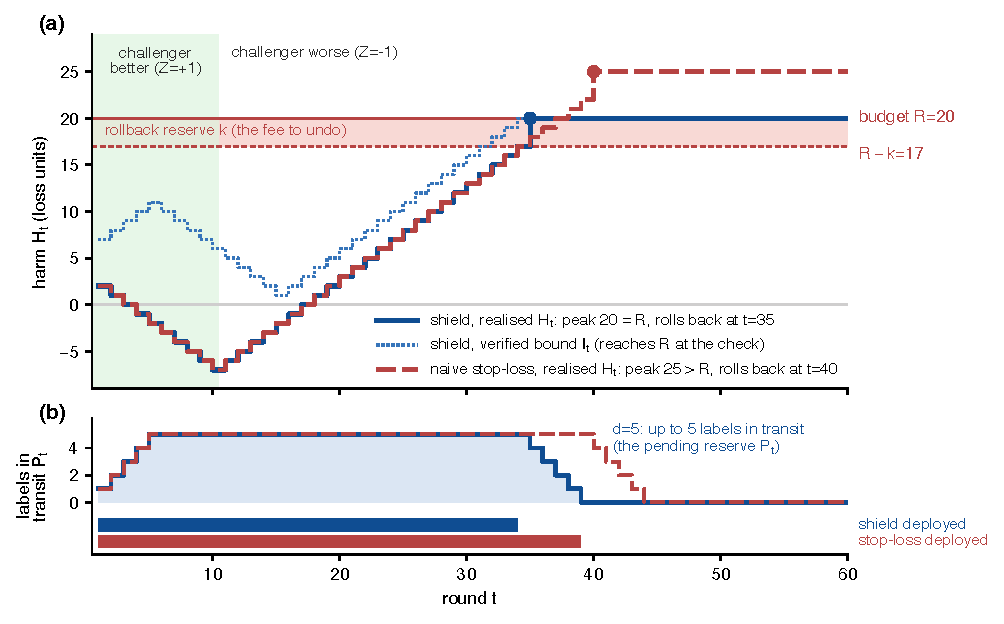
\includegraphics[width=\linewidth]{figures/fig_mechanism.pdf}
\caption{The shield stays within the budget on a tape where a naive stop-loss overshoots it. Tape: 60 rounds, every round a disagreement, the challenger better ($Z=+1$) for the first 10 rounds and worse ($Z=-1$) afterwards, label delay $d=5$, fee $k=3$, budget $R=20$, inner rule always-challenger. (a) Realised harm $H_t$ of the shield (solid) and of a stop-loss that rolls back when fees plus resolved harm exceed $R-k$ (dashed), with the shield's check (dotted; fees, rollback reserve $k$, resolved and pending harm, cf.\ $W_t$ in Section~\ref{sec:method}), evaluated after round $t$ (shaded band between $R-k$ and $R$). The shield rolls back at round 35 with peak harm exactly 20; the stop-loss, blind to the five labels in transit and to the rollback fee, rolls back at round 40 with peak harm 25. (b) Labels in transit and rounds on which each controller is deployed. Both traces are computed by running the committed code on this tape.}
\label{fig:mechanism}
\end{figure}


\begin{table}[t]
\caption{Running example ($k=\ExK$, $R=\ExR$, $d=\ExD$, full sampling, every round exposed, promotion at round 1): the check $W$ at the $n$-th exposed round on a tape where every round is harmful and on one where every round benefits the challenger.}\label{tab:example}
\centering\small
\begin{tabular}{@{}rrlrl@{}}
\toprule
exposed round $n$ & $W$, all-harm tape & decision & $W$, all-benefit tape & decision \\
\midrule
1 & 7 & deploy & 7 & deploy \\
5 & 11 & deploy & 11 & deploy \\
6 & 12 & deploy & 10 & deploy \\
10 & 16 & deploy & 6 & deploy \\
14 & 20 & deploy & 2 & deploy \\
15 & 21 & roll back & 1 & deploy \\
\bottomrule
\end{tabular}

\end{table}

\begin{algorithm}[t]
\caption{One round of the risk-budget shield}\label{alg:shield}
\begin{algorithmic}
\STATE \textbf{Input:} inner rule, budget $R$, level $\delta$, menu of rates, label reserve $L_{\rm res}$
\STATE Release labels; update $A,P,V,n_{\rm b},N_{t-1}$
\IF{$a_{t-1}=1$ \textbf{and} $kN_{t-1}+n_{\rm b}+A+P+D_\delta(V)+T-t+1\le R$}
  \STATE \textbf{ride-out:} $a_t\leftarrow1$, no query, $n_{\rm b}\leftarrow n_{\rm b}+g_t$; \textbf{return} \COMMENT{stays on until $T$; no rollback reserve}
\ENDIF
\STATE Show the inner rule the label balance minus $L_{\rm res}$ if $a_{t-1}=0$, the full balance otherwise
\STATE $(\tilde a_t,\tilde q_t)\leftarrow$ inner rule's proposal and query decision
\IF{$\tilde a_t=0$}
  \STATE $a_t\leftarrow0$ \COMMENT{rollback fee already reserved}
  \STATE query $q_t\leftarrow\tilde q_t$ if $a_{t-1}=0$, else $q_t\leftarrow0$ \COMMENT{inner rule's query passes through}
\ELSE
  \STATE choose the cheapest $\pi$ in the menu with $W_t(\pi)\le R$ (else $\pi=1$; blind if no labels remain)
  \IF{$W_t(\pi)\le R$} \STATE $a_t\leftarrow1$; if $g_t=1$ draw $q_t\sim\mathrm{Bern}(\pi)$ \COMMENT{shield owns the query}
  \ELSE \STATE $a_t\leftarrow0$; $q_t\leftarrow\tilde q_t$ if $a_{t-1}=0$, else $q_t\leftarrow0$ \COMMENT{veto, or forced rollback}
  \ENDIF
\ENDIF
\end{algorithmic}
\end{algorithm}

\begin{table}[t]
\caption{Variants of the shield. All use the same check $W_t\le R$; they differ in how exposed rounds are monitored. Frozen settings are in Appendix Table~\ref{tab:arms}.}\label{tab:variants}
\centering\small
\begin{tabular}{@{}p{2.5cm} p{5.3cm} p{2.6cm} p{3.9cm}@{}}
\toprule
Variant & What it changes & Guarantee & Use when \\
\midrule
Full sampling & $\pi=1$ on every exposed round; each pending round booked at 1; no martingale term & $\sup_tH_t\le R$ surely ($\delta=0$) & labels cover the exposed rounds, or a deterministic guarantee is required \\
Paced with settlement & $\pi$ from labels remaining per expected exposed round, floor $\pi_{\min}$; a sampled round is booked at 1 until a settlement window has passed, then enters the inverse-propensity sum and the exact-coin mixture & probability $\ge1-\delta$ & labels are fewer than exposed rounds and $\delta>0$ is acceptable \\
Blind-round & $\pi\in\{1,\text{blind}\}$; a round is left without a query, booked at 1, when the headroom left after booking it is at least a margin & $\sup_tH_t\le R$ surely (with $\pi_{\min}=1$) & headroom is large relative to the exposure in one delay window, so blind rounds are affordable \\
Label-scarce (v3) & paced variant with a lower floor $\pi_{\min}$, a wider mixture grid, and no blind rounds; designed after the real-stream run for $T=2000$, $B=200$ & probability $\ge1-\delta$ & exposed rounds far outnumber labels and $h$ is large; no help at small $h$ \\
\bottomrule
\end{tabular}
\end{table}

\section{Guarantees}\label{sec:theory}
\begin{theorem}[Pathwise risk budget]\label{thm:main}
Under O1--O4, for any inner policy, any tape and any $R\ge0$, the shield satisfies $\PP(\sup_tH_t>R)\le\delta$. If $\pi_t=1$ on every monitored round, $\sup_tH_t\le R$ surely.
\end{theorem}
\begin{proof}
\emph{Step 1: a pathwise bound.} For exposed rounds $s\le t$: a blind round has $\chi_s\le1$. For a monitored round, $\chi_s=\chi_sq_s/\pi_s+\xi_s$ with $\xi_s=\chi_s(1-q_s/\pi_s)$, and $\chi_sq_s/\pi_s$ equals $\chi_s/\pi_s$ if the round is queried and released, is at most $1/\pi_s$ if queried and pending, and is $0$ if not queried. Rounds that are not exposed have $\chi_s=0$. Hence $\sum_{s\le t}\chi_s\le n_{\rm b}+A+P+M_t$.

\emph{Step 2: the check dominates the harm.} Let $E$ be the event of Lemma~\ref{lem:bennett} (or Lemma~\ref{lem:coin} for the paced variant), which has probability at least $1-\delta$ and is sure when $\pi\equiv1$. Fix a round $t$ with $a_t=1$ and proposed rate $\pi_t$. The fees paid through $t$ are $k(N_{t-1}+\one\{a_{t-1}=0\})$. By Step 1 the excess loss of rounds $s\le t-1$ is at most $n_{\rm b}+A+P+M_{t-1}$. Round $t$ adds at most $g_t\kappa(\pi_t)$ to $n_{\rm b}+A+P$ (a blind round is at most $g_t$, a monitored round satisfies $\chi_tq_t/\pi_t\le g_t/\pi_t$) and $g_t(1/\pi_t-1)$ to $V$. On $E$, $M\le D_\delta(V)$ with $D_\delta$ nondecreasing, so $H_t+k\le W_t(\pi_t)$. The shield deploys only if $W_t(\pi_t)\le R$, hence $H_t\le R-k$ at every deployed round on $E$. In the ride-out branch, on $E$ the harm through round $t-1$ plus at most one unit per later round stays below $R$, so $H_s\le R$ for every $s\ge t$ directly.

\emph{Step 3: rollbacks.} Take any $t$ and let $t'\le t$ be the last deployed round; if there is none, $H_t=0\le R$. If $t'$ is a ride-out round the shield stays deployed to $T$, so $t=t'$ and Step 2 applies. Otherwise $H_{t'}\le R-k$. If $t=t'$ we are done. If not, the controller rolls back at $t'+1$, paying $k$, and makes no further action change through $t$ because a later deployment would contradict the choice of $t'$; also $\chi_s=0$ whenever $a_s=0$. So $H_t=H_{t'}+k\le R$. No monotone invariant is needed.

Therefore $\sup_tH_t\le R$ on $E$ and $\PP(\sup_tH_t>R)\le\PP(E^c)\le\delta$. With $\pi\equiv1$, $V\equiv0$ and $M\equiv0$, so the bound is deterministic. The argument needs only that some valid upper bound on $H_t+k$ is verified at each deployed round, so it also covers the sharper bound of Appendix~\ref{app:v2}.
\end{proof}
In words: whatever the losses do and however the labels are delayed or withheld, the shield's harm exceeds $R$ in at most a fraction $\delta$ of its own runs; with full sampling it never does. The randomness is the shield's, not the world's, so no model of the world has to be believed.

\begin{proposition}[Both reserves are necessary]\label{prop:reserves}
Suppose every label requested at round $s$ is released no earlier than $s+d$, $d\ge1$, and a controller satisfies the $(R,\delta)$ budget on every tape. Fix an environment $\mathcal E$ and rounds $j$, $m$ with $1\le m\le d$. Let $\mathcal A$ be the event that the first promotion is at round $j$ and $a_s=1$ for $s=j,\dots,j+m-1$; let $e$ and $n$ be the numbers of disagreement rounds in $[j,j+m-1]$ and $[j,T]$. If $\PP_{\mathcal E}(\mathcal A)>\delta$ then $R\ge\min(2k+e,\,k+n)$.
\end{proposition}
\begin{proof}
Let $\mathcal E'$ coincide with $\mathcal E$ on all rounds before $j$ (losses, flags, delays) and have $Z_s=-1$ on every later disagreement round (so $\ell_s(0)=0$, $\ell_s(1)=1$), with the same flags. A label visible at a round $s\le j+d-1$ was requested at or before $s-d\le j-1$, where the two environments coincide. With the same coins the controller therefore takes the same actions through round $j+d-1$ in both environments. Since $m\le d$, the event $\mathcal A$ is determined by actions through $j+m-1\le j+d-1$, so $\PP_{\mathcal E'}(\mathcal A)=\PP_{\mathcal E}(\mathcal A)>\delta$.

Under $\mathcal E'$ every $\chi_s\ge0$, and $\chi_s=1$ on disagreement rounds with $a_s=1$, so $H_t$ never decreases. On $\mathcal A$, $H_{j-1}=0$ and $H_{j+m-1}=k+e$. If the controller later rolls back at round $\rho$, then $H_\rho\ge k+e+k=2k+e$. If it never rolls back after $j$, then $a_s=1$ for all $s\ge j$ and $H_T=k+n$. Since $n\ge e$, $\sup_tH_t\ge\min(2k+e,\,k+n)$ on $\mathcal A$. If $R<\min(2k+e,k+n)$ this gives $\PP_{\mathcal E'}(\sup_tH_t>R)\ge\PP_{\mathcal E'}(\mathcal A)>\delta$, contradicting validity. Hence $R\ge\min(2k+e,k+n)$.
\end{proof}

In words: no valid controller can hold a new promotion through a feedback-blind window of more than $R-2k$ exposed rounds, because on the tape that turns every such round into harm it would have paid the promotion fee, the harm of the window, and the fee to leave. The three terms of $W_t$ on a first promotion are exactly these: $k$ for the promotion, $k$ reserved for the rollback, and one unit per exposed round whose label cannot yet have arrived. On an all-disagreement, all-harm tape the full-sampling shield holds a first promotion for exactly $\lfloor R-2k\rfloor$ exposed rounds (Appendix~\ref{app:proofs}), which is the most Proposition~\ref{prop:reserves} allows when $d\ge\lfloor R-2k\rfloor$. This was checked by simulation in \PThreeAttain{} of \PThreeCells{} $(d,R)$ cells (Appendix Table~\ref{tab:prop3}). The ride-out branch matches the $k+n$ term, using the remaining round count as an upper bound on $n$. The proposition concerns the feedback-blind window only.

\emph{Running example.} With $k=\ExK$ and $R=\ExR$ if labels took at least $\ExRoll$ rounds to return ($d\ge\ExRoll$), the proposition would say that holding $\ExRoll$ exposed rounds before any label arrives needs $R\ge2k+\ExRoll=\ExNeedR$, so no valid controller can hold more than $R-2k=\ExH$. The shield of Section~\ref{sec:method} holds exactly $\ExHold$ (Table~\ref{tab:example}), so in a feedback-blind window it gives up nothing. With the example's $d=\ExD$ only the first $\ExD$ rounds of the hold are blind in this sense, and on the all-harm tape the labels that come back afterwards bring no relief; when they show gains, $W$ falls and the hold continues, as in the last column of the table.

\begin{proposition}[Ruin bound for a first spell]\label{prop:price}
Take the full-sampling shield with fixed delay $d$ during its first deployment spell, while labels remain and the inner rule keeps proposing the challenger. Let $y_1,y_2,\dots$ be the values of $Z$ on the exposed rounds in order, with $\E[y_i\mid\text{past}]\ge\mu>0$, and let $m=R-2k-d$. Then $\PP(\text{forced rollback in the spell})\le e^{-2\mu m}$. If $y_i\in\{-1,+1\}$ with $\PP(y_i=+1\mid\text{past})\ge p>\tfrac12$, the probability is at most $((1-p)/p)^{\lfloor m\rfloor+1}$.
\end{proposition}
\emph{Proof sketch.} During the spell $W_t\le2k+d-S_n$ with $S_n=y_1+\dots+y_n$, because the pending rounds and the current round number at most $d$ and the released rounds form a prefix of the exposed sequence. A forced rollback needs $S_n<-m$ for some $n$, and $e^{-2\mu S_n}$ (respectively $(q/p)^{S_n}$) is a nonnegative supermartingale, so Ville's inequality gives the bounds. The full proof is in Appendix~\ref{app:proofs}. \hfill$\square$

In words: if the challenger is right more often than not, the shield is forced out of its first deployment only with a probability that falls exponentially in $m=R-2k-d$. The intuition for $m$ is the following. During the first spell the check is at most $2k+d-S_n$: $2k$ is the promotion and rollback fees, $d$ is the most that can be in transit (the pending rounds and the current one) at one time, and $S_n$ is the net gain banked on rounds whose labels have come back. The shield is forced out only when $2k+d-S_n>R$, that is when the net gain falls below $-m$. So $m$ is the cushion that the budget leaves after paying both fees and covering a full delay window of unseen rounds, and the bound is the probability that a random walk with positive drift ever sinks below $-m$. \emph{Running example:} $m=\ExR-2\cdot\ExK-\ExD=\ExM$. If the challenger is right on $70\%$ of exposed rounds with $\pm1$ steps ($p=.7$, $\mu=.4$), the first spell is cut short with probability at most $(3/7)^{10}\approx\ExBoundTwo$, and $e^{-2\mu m}\approx\ExBoundExp$.

We checked Proposition~\ref{prop:price} by simulation in \PFourCells{} cells ($p\in\{.6,.7,.8\}$, $d\in\{1,5\}$, $R\in\{10,12,15,20\}$): all lie within Monte Carlo error of the bound. At $d=1$ the bound is close to the simulated frequency (\PFourTightEmp{} against \PFourTightBound{} at $p=.6,R=10$; \PFourTightEmpB{} against \PFourTightBoundB{} at $p=.7,R=10$). At $d=5$ it is looser because the pending count is usually below $d$ (Appendix Table~\ref{tab:prop4}).

\paragraph{What the bound predicts.}
Let $r$ be the disagreement rate while deployed and $h=R-2k$ the headroom. Proposition~\ref{prop:reserves} limits any valid controller to holding a first promotion for at most $h$ exposed rounds before any label has arrived, and one delay window contains about $rd$ of them. In the running example every round is a disagreement round, so $r=1$ and $x=rd/h=\ExD/\ExH\approx\ExX$.
When $x=rd/h$ is small, a promotion can be held until labels arrive and the shield can behave like the unconstrained rule.
When $x>1$, no valid controller can remain deployed through one delay window on the strength of the prior alone, and it must cycle (deploy, roll back, wait, re-enter) until gains banked from released labels cover the window.

We state the following as a prediction that we derive informally from Proposition~\ref{prop:reserves}; it is not a corollary, because the proposition covers only the first promotion and says nothing about later spells. The share $L$ of the unconstrained rule's improvement that the shield gives up increases with $x$, is small for $x<.5$, and is near one for $x>1$. The prediction was committed with its test script before the test was first run, and is evaluated in Section~\ref{sec:regimemap}. In words: when one delay window holds only a small fraction of the headroom, the shield behaves almost like the unconstrained rule; when it holds more than the headroom, the shield cannot bank gains fast enough and keeps little of the benefit.

\section{Experiments}\label{sec:exp}
\paragraph{How harm is scored.}
Every controller, whether or not it was designed around a budget, is scored by the same quantity: the realised harm $\sup_tH_t$ of its run against never switching, computed after the run from the full tape, including the losses of unlabelled rounds that the controller never sees. Never switching has $H_t\equiv0$ and so keeps every budget; the question for controllers that also keep the budget is therefore whether they still beat doing nothing, which is why tables report cost $J$ ``vs never''. A comparator \emph{exceeds} the budget when $\sup_tH_t>R$. Only the stop-loss is told $R$, so for the other comparators this measures the absence of a guarantee rather than a design flaw: a team that wants a budget $R$ has no way to enforce it with them.

\paragraph{Scenario settings.}
The settings are not chosen for this study. $T=300$, $B=60$, $k=3$ and $c_q=.05$ are the defaults of the programme's simulator (\texttt{regimes\_v1.json}) used by earlier work in the same programme. $T=2000$ is the length of the cached real-stream episodes, and $B=200$, $k=5$, $c_q=.05$ are the programme's existing real-stream scenario, taken over unchanged; budgets are restated in headroom terms $R=2k+h$, with $h=50$ and $100$ added because the horizon is $6.7$ times longer. None of these settings was tuned in this study.

\paragraph{Simulation.}
The registered confirmation (frozen before any confirmation seed was opened) uses the 24 regimes of the original family and 6 stress regimes built to stress delayed and missing feedback (adverse informative delay, dropout of unfavourable labels, a bait-and-reverse path, dependence $\rho=.95$), with $T=300$, label budget $B=60$, $k=3$, $c_q=.05$ and $\NSeedsPerRegime$ seeds per regime ($\NRunsPerArm$ runs per arm), run once. A regime fixes the probability $p(t)$ that the challenger is right when the models disagree, the disagreement rate $r$, the serial dependence $\rho$ and a delay mechanism; the generator and all 30 regimes are described in Appendix~\ref{app:sim} (Table~\ref{tab:regimes_app}).
The inner rule is Wald with cutoff tuned by a 32-configuration random search on separate seeds, with the same search budget as every comparator. Budgets are $R\in\{12,20,30\}$, that is $h\in\{6,14,24\}$. The cost $J$ is deployed loss plus label, switching and compute fees.
Comparators are tuned Wald with cutoff, two-sided CUSUM, a betting e-process gate over Wald, Wald with cutoff and a one-sided CUSUM rollback, and a naive stop-loss (Wald with cutoff that rolls back when fees plus resolved harm exceed $R-k$, with no pending reserve and no width). None is a native-source reproduction: Wald with cutoff is a documented adapter and the others are in-house heuristics. Appendix~\ref{app:comp} describes each precisely and lists the frozen parameters (Table~\ref{tab:comp}).

\paragraph{Stress regimes.}
The six stress regimes were written by us, from the design document and before any run of the shield, to stress the failure mode that the reserves address: labels unfavourable to the challenger arrive 40 rounds late (adverse informative delay); $30\%$ of requested labels never arrive (label dropout); unfavourable labels are dropped with probability $.6$, so that the released labels look favourable (adverse dropout); the challenger is strongly better in the first quarter and then strongly worse (bait and reversal); and a worse challenger, or a bait path, under dependence $\rho=.95$. They are favourable to the shield by construction, which is why every comparison is also reported on the 24 original regimes alone.

\paragraph{Real streams.}
We use 14 cached streams of paired 0/1 losses (230 episodes, $T=2000$, $B=200$, $k=5$, 20 policy seeds per episode; Appendix Table~\ref{tab:streams} gives the source, task, models, episodes, delay and error rates of each), under the stream's own delay (clean), adverse dropout (unfavourable labels never released with probability $.6$) and adverse delay (unfavourable labels delayed by 400 further events); the two corrupted conditions change only the feedback. The delays are simulated constants on the event clock (the label of event $t$ is released at event $t+d$), not authentic label-release times, which the cached streams do not carry; the corruptions are likewise simulated, drawn once per stream, episode and condition independently of the policy seeds. Budgets are $R=10+h$ with $h\in\{6,14,24,50,100\}$. Every arm is frozen from simulation and none was run or tuned on these streams before this study. The challenger is worse on two streams (airlines, bank) and better on twelve.

\paragraph{What the policy seeds randomise.}
Only the controllers' coins: the shield's query coins $q_t$ (assumption O2), and the paced-acquisition coins of the inner rule and of the comparators. In the real-stream study the tape (losses, flags, delays and corruptions) of an episode is fixed, so the 20 policy seeds per episode change nothing but these coins, and runs of one episode are not independent evidence about the stream. In the simulation the tape seed also seeds the controllers' coins, one run per tape, so a seed varies the tape and the coins together; all arms see the same tape.

\begin{table}[t]
\caption{Registered confirmation C1--C6 (simulation, \NRunsPerArm{} runs per arm). Source: \texttt{confirm\_summary.json}.}\label{tab:confirm}
\centering\small
\resizebox{\linewidth}{!}{\begin{tabular}{@{}l p{4.8cm} p{7.2cm} l@{}}
\toprule
ID & Registered statistic & Result & Verdict \\
\midrule
C1 & Full-sampling shield, $R\in\{12,20,30\}$, and blind-round variant: violations of $R$ & 0 / 30{,}000 in each of 4 arms; per-regime Wilson upper $\le 0.004$ & supported \\
C2 & Paced shield, $\delta=.05$, $R\in\{20,30\}$: violations & 1 and 1 / 30{,}000; largest per-regime Wilson upper 0.006 & supported \\
C3 & Five comparators, worst-regime exceedance of $R=20$ (Wilson lower bound) & all five above $.05$; smallest lower bound 0.605 & supported \\
C4 & Pooled $\Delta J$ of the $R=20$ shield, 95\% CI & vs never $-$2.10 [$-$2.22, $-$1.98]; vs Wald+cutoff +0.96 [+0.86, +1.06] & supported \\
C5 & $\Delta J$ vs Wald+cutoff, 6 stress regimes (24 original regimes) & $-$5.19 [$-$5.40, $-$4.98] (+2.50) & supported \\
C6 & Ablations at $R=12$, worst-regime violation rate (no pending / no rollback reserve / no width) & 0.940 / 0.862 / 0.341 & supported \\
\bottomrule
\end{tabular}
}
\end{table}

\begin{table}[t]
\caption{Simulation, $R=20$, pooled over \NRegimes{} regimes. $J$ is mean cost; ``vs never'' is the relative difference in $J$; harm quantiles are of $\sup_tH_t$. The last two columns give the exceedance rate of $R=20$ pooled and in the worst regime. The two shields keep the budget; the comparators do not.}\label{tab:sim}
\centering\scriptsize
\resizebox{\linewidth}{!}{\begin{tabular}{@{}p{4.4cm} r r r@{}}
\toprule
Controller & $J$ & vs never (\%) & labels \\
\midrule
Never switch & 71.53 & +0.0 & 0.0 \\
Wald+cutoff (tuned) & 68.47 & $-$4.3 & 38.8 \\
CUSUM (tuned) & 68.97 & $-$3.6 & 47.0 \\
E-process gate (tuned) & 71.89 & +0.5 & 49.7 \\
CUSUM rollback, $\theta=8$ & 68.62 & $-$4.1 & 49.8 \\
Stop-loss, $R=20$ & 68.79 & $-$3.8 & 49.8 \\
\midrule
Shield, full sampling, $R=20$ & 69.43 & $-$2.9 & 44.2 \\
Shield, paced, $R=20$, $\delta=.05$ & 69.80 & $-$2.4 & 37.8 \\
\bottomrule
\end{tabular}\par\smallskip
{\setlength{\tabcolsep}{4pt}\begin{tabular}{@{}p{4.5cm} r r r p{3.0cm} p{2.3cm}@{}}
\toprule
Controller & $q_{99}$ harm & max harm & pooled viol. (\%) & worst rate [Wilson] & worst regime \\
\midrule
Never switch & 0 & 0 & 0.0 & 0.000 & -- \\
Wald+cutoff (tuned) & 37 & 59 & 6.6 & 0.852 [0.829, 0.873] & Adverse dropout \\
CUSUM (tuned) & 34 & 117 & 7.9 & 0.987 [0.978, 0.992] & High switch fee \\
E-process gate (tuned) & 33 & 57 & 4.3 & 0.635 [0.605, 0.664] & Adverse dropout \\
CUSUM rollback, $\theta=8$ & 35 & 71 & 4.4 & 0.830 [0.805, 0.852] & Adverse dropout \\
Stop-loss, $R=20$ & 34 & 59 & 4.2 & 0.841 [0.817, 0.862] & Adverse dropout \\
\midrule
Shield, full sampling, $R=20$ & 20 & 20 & 0.000 & 0.000 [0.000, 0.004] & -- \\
Shield, paced, $R=20$, $\delta=.05$ & 16 & 22 & 0.003 & 0.001 [0.000, 0.006] & Bait reversal \\
\bottomrule
\end{tabular}}
}
\end{table}

\subsection{The budget holds and the comparators break it}
Table~\ref{tab:confirm} lists the six registered outcomes, all supported.
The full-sampling shield and the blind-round variant had \COneTotal{} violations in each of four arms ($R\in\{12,20,30\}$ and the variant). The paced shield with $\delta=.05$ had \CTwoTotal{} violations in two arms, against the guaranteed rate of $.05$, and the largest per-regime Wilson upper bound over all six arms is \CTwoMaxHi.

Table~\ref{tab:sim} shows the comparators at $R=20$: each exceeds the budget in the majority of runs in its worst regime (Wald with cutoff \WorstWald, CUSUM \WorstCusum, gate \WorstGate, CUSUM rollback \WorstCusumRb, stop-loss \WorstStop).
The worst-regime figure overstates typical behaviour, so we give the pooled rates alongside. The exceedance is concentrated in the stress regimes: pooled (mean of per-regime rates) over the six stress regimes, Wald with cutoff exceeds $R=20$ in \StressExceedWald\% of runs and over the 24 original regimes in \OrigExceedWald\% (CUSUM \StressExceedCusum\% and \OrigExceedCusum\%; stop-loss \StressExceedStop\% and \OrigExceedStop\%; Table~\ref{tab:split}). Over the five comparators the original-regime rates range from \OrigExceedMin\% to \OrigExceedMax\%. Figure~\ref{fig:violations} shows the exceedance in every regime and the corresponding counts on the real streams.

\begin{figure}[!htbp]
\centering
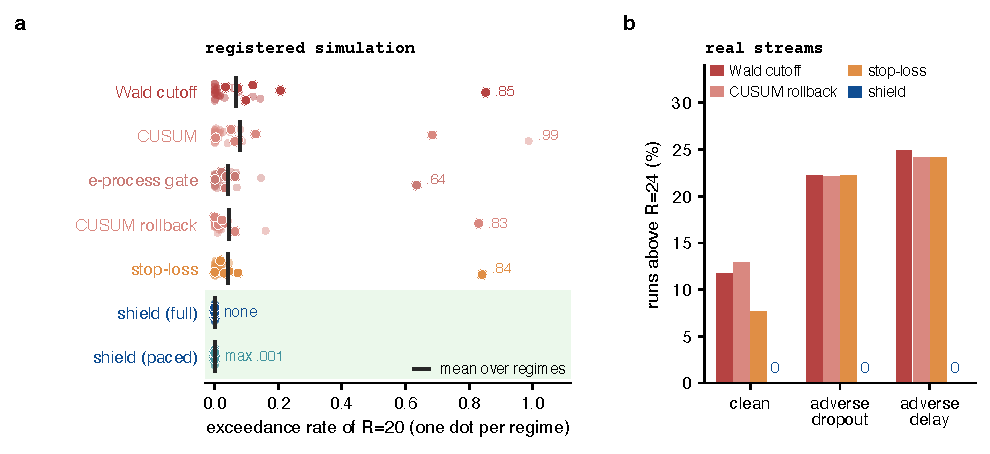
\includegraphics[width=\linewidth]{figures/fig_violations.pdf}
\caption{The tuned comparators often exceed the budget in stress regimes and on real streams with corrupted feedback. (a) Exceedance rate of $R=20$ in each of the \NRegimes{} registered regimes, based on \NSeedsPerRegime{} seeds per regime; stress regimes are marked $*$ and set below the line. The full-sampling shield has no observed violations; the two paced variants have \CTwoTotal{} in total, one per arm, including one run in bait reversal. (b) Real streams: runs, out of \RealRunsPerArm{} per arm and condition, with harm above $R=24$ (the arms' own budget at $h=14$ for stop-loss and the shield). The shield arms have \RealShieldViolClean{} in every condition.}
\label{fig:violations}
\end{figure}

Even there none carries a guarantee, whereas the shield's violation count is \COneTotal{} for full sampling and \CTwoTotal{} for the paced arms in total.

The two comparators that try to keep a budget, the stop-loss and the CUSUM rollback, fail in the same regimes as the rules they wrap, because the harm of rounds whose labels are in transit and the rollback fee are invisible to them.
The ablations indicate that each part of the accounting is needed: without the pending reserve the worst-regime violation rate at $R=12$ is \AblNoPending, without the rollback reserve \AblNoRollback, and without the confidence width \AblNoConf{} (Table~\ref{tab:ablation}).

Among controllers that keep the budget, the shield beats never switching: at $R=20$ the pooled cost is \JFthreeTwenty{} against \JNever{} for never switching, a difference of \SimVsNeverDelta{} with 95\% interval [\SimVsNeverLo, \SimVsNeverHi], or \SimVsNeverPct\%. In the six stress regimes, where delayed and missing feedback mislead the heuristics, the shield also has lower cost than tuned Wald with cutoff by \StressDelta{} ([\StressLo, \StressHi], \StressPct\%). Figure~\ref{fig:cost_tail} places every arm by mean cost and 99th-percentile harm.

\begin{figure}[!htbp]
\centering
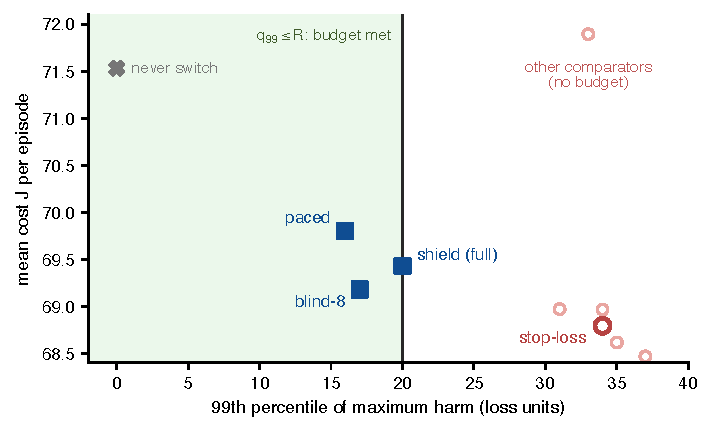
\includegraphics[width=\linewidth]{figures/fig_cost_tail.pdf}
\caption{Tail-risk diagnostic for the registered run (\NRegimes{} regimes, \NSeedsPerRegime{} seeds each): mean cost $J$ against the 99th percentile $q_{99}$ of maximum harm. Panels group arms by budget $R=12,20,30$; the vertical line is $R$ and the shaded region is $q_{99}\le R$. Filled markers satisfy this quantile check; open markers do not, including the stop-loss and the three reserve/width ablations. This 99th-percentile diagnostic does not replace the time-uniform violation guarantee. Never switching has zero harm but pooled $J=\JNever$, about 3 above tuned Wald with cutoff ($J=\JWald$); the budget-free comparators (faint circles: Wald with cutoff, CUSUM, CUSUM rollback, e-process gate) have $q_{99}$ between 31 and 37.}
\label{fig:cost_tail}
\end{figure}


\begin{table}[t]
\caption{Exceedance rate of $R=20$ pooled (mean of per-regime rates) over the six stress regimes and the 24 original regimes.}\label{tab:split}
\centering\small
\begin{tabular}{@{}l r r@{}}
\toprule
Arm & 6 stress regimes & 24 original regimes \\
\midrule
Wald with cutoff & 0.231 & 0.025 \\
CUSUM & 0.168 & 0.056 \\
E-process gate & 0.132 & 0.020 \\
CUSUM rollback ($h=8$) & 0.160 & 0.015 \\
Stop-loss ($R=20$) & 0.168 & 0.011 \\
Full shield ($R=20$) & 0.000 & 0.000 \\
Paced shield ($R=20$) & 0.000 & 0.000 \\
\bottomrule
\end{tabular}

\end{table}

\begin{table}[t]
\caption{Ablations at $R=12$ (registered C6): worst-regime violation rate with the Wilson 95\% interval.}\label{tab:ablation}
\centering\small
\begin{tabular}{@{}l l r l@{}}
\toprule
Ablation ($R=12$) & worst regime & rate & Wilson 95\% \\
\midrule
no pending reserve & Adverse dropout & 0.940 & [0.924, 0.953] \\
no rollback reserve & Adverse dropout & 0.862 & [0.839, 0.882] \\
no confidence width & Bait reversal & 0.341 & [0.312, 0.371] \\
\bottomrule
\end{tabular}

\end{table}

\subsection{Calibrated comparators}\label{sec:calib}
[RESULTS PENDING: calibrated stop-loss and CUSUM rollback, see calib\_summary.json]

\begin{table}[t]
\caption{Real streams, pooled over 14 streams (equal weight), \RealRunsPerArm{} runs per arm and condition. $J$ is mean cost per episode, ``vs never'' the difference in $J$, ``viol.'' the number of runs above the budget: $R=24$ for the comparators, the arm's own $R$ ($24$, $60$ or $110$) for the shield and stop-loss. Source: \texttt{real\_tables.md}.}\label{tab:real}
\centering\scriptsize
\resizebox{\linewidth}{!}{\begin{tabular}{@{}l r r r r r r r r r @{}}
\toprule
 & \multicolumn{3}{c}{Clean} & \multicolumn{3}{c}{Adverse dropout} & \multicolumn{3}{c}{Adverse delay} \\
\cmidrule(lr){2-4}\cmidrule(lr){5-7}\cmidrule(lr){8-10}
Controller & $J$ & vs never & viol. & $J$ & vs never & viol. & $J$ & vs never & viol. \\
\midrule
Never switch & 602.19 & 0.0 & 0 & 602.19 & 0.0 & 0 & 602.19 & 0.0 & 0 \\
Wald+cutoff & 422.60 & $-$179.6 & 456 & 427.79 & $-$174.4 & 863 & 440.16 & $-$162.0 & 966 \\
CUSUM & 438.33 & $-$163.9 & 650 & 434.68 & $-$167.5 & 834 & 447.45 & $-$154.7 & 968 \\
E-process gate & 438.46 & $-$163.7 & 417 & 427.04 & $-$175.1 & 593 & 442.07 & $-$160.1 & 1{,}080 \\
CUSUM rollback $\theta=8$ & 435.16 & $-$167.0 & 502 & 437.40 & $-$164.8 & 857 & 485.17 & $-$117.0 & 937 \\
Stop-loss, $R=24$ & 439.33 & $-$162.9 & 298 & 436.11 & $-$166.1 & 863 & 469.90 & $-$132.3 & 936 \\
\midrule
Shield, full, $R=24$ & 519.92 & $-$82.3 & 0 & 518.75 & $-$83.4 & 0 & 521.50 & $-$80.7 & 0 \\
Shield, paced, $R=24$ & 510.37 & $-$91.8 & 0 & 510.29 & $-$91.9 & 0 & 511.86 & $-$90.3 & 0 \\
Shield, full, $R=60$ & 502.29 & $-$99.9 & 0 & 499.91 & $-$102.3 & 0 & 505.49 & $-$96.7 & 0 \\
Shield, paced, $R=60$ & 455.29 & $-$146.9 & 0 & 452.98 & $-$149.2 & 0 & 456.21 & $-$146.0 & 0 \\
Shield, paced, $R=110$ & 441.82 & $-$160.4 & 0 & 440.95 & $-$161.2 & 0 & 447.62 & $-$154.6 & 0 \\
\bottomrule
\end{tabular}
}
\end{table}

\subsection{Real streams}
Table~\ref{tab:real} gives the pooled results. The shield had \RealShieldViolClean{} violations of its own budget in every arm, headroom and condition (\RealRunsPerArm{} runs each).
Tuned Wald with cutoff exceeded $R=24$ in \RealWaldExceedClean{} runs on clean feedback, \RealWaldExceedDropout{} under adverse dropout and \RealWaldExceedDelay{} under adverse delay, with a largest harm of \RealWaldMaxClean, \RealWaldMaxDropout{} and \RealWaldMaxDelay{} against a budget of 24. The stop-loss broke its own $R=24$ in \RealStopExceedClean, \RealStopExceedDropout{} and \RealStopExceedDelay{} runs.
The shield improves on never switching by \RealPiVsNeverCleanHfourteen{} to \RealPiVsNeverCleanHhundred{} cost units per episode with full sampling at $h=14$ to $100$ on clean feedback, and by more with paced sampling at large headroom. At $h=6$ the budget leaves almost no room (a promotion holds for $\lfloor R-2k\rfloor=6$ exposed rounds), and the shield is within \RealSixVsNever{} units of never switching.

Table~\ref{tab:harm} isolates the two streams on which the challenger is worse. Under corrupted feedback, the shield has lower cost than tuned Wald with cutoff by \HarmDropMin{} to \HarmDropMax{} units under dropout and \HarmDelayMin{} to \HarmDelayMax{} under delay. The corrupted feedback withholds the labels that would reveal the harm, and Wald with cutoff, which sees only released labels, keeps the challenger deployed. The shield remains above never switching there, by \HarmNeverMin{} to \HarmNeverMax{} units under corrupted feedback, since the budget permits some harm before the shield withdraws.

\begin{table}[t]
\caption{Two harmful streams (airlines, bank): $\Delta J$ of the full-sampling shield against Wald with cutoff and against never switching, by headroom $h$.}\label{tab:harm}
\centering\scriptsize
\resizebox{\linewidth}{!}{\begin{tabular}{@{}l l r r r r r @{}}
\toprule
 & & \multicolumn{5}{c}{headroom $h$ ($R=10+h$)} \\
\cmidrule(lr){3-7}
Feedback & vs & 6 & 14 & 24 & 50 & 100 \\
\midrule
Clean & wald\_cut & +2.2 & +2.3 & +0.9 & +2.6 & +6.2 \\
 & never & +10.9 & +11.0 & +9.6 & +11.3 & +14.9 \\
Adverse dropout & wald\_cut & $-$54.5 & $-$52.6 & $-$51.5 & $-$42.0 & $-$32.9 \\
 & never & +13.4 & +15.3 & +16.4 & +25.9 & +35.0 \\
Adverse delay & wald\_cut & $-$87.5 & $-$84.3 & $-$81.2 & $-$66.8 & $-$45.5 \\
 & never & +16.9 & +20.0 & +23.2 & +37.6 & +58.8 \\
\bottomrule
\end{tabular}
}
\end{table}

\subsection{Regime map}\label{sec:regimemap}
We tested the prediction of Section~\ref{sec:theory} on the label-scarce simulation family and on the ten real streams where Wald with cutoff gains at least 10\% of $J$(never) (\NUnits{} units of regime or stream, arm and headroom). Table~\ref{tab:regime} reports Spearman correlations between $x=rd/h$ and $L=(J_{\rm shield}-J_{\rm Wald})/(J_{\rm never}-J_{\rm Wald})$ with regime- or stream-bootstrap intervals, and the median of $L$ by bin of $x$.
All \RegimeTestsSupported{} of \RegimeTestsTotal{} pre-stated tests are supported, with correlations from \SpearLo{} to \SpearHi.

For the paced arms the median $L$ is small below $x=.5$, so the shield retains \KeepLo--\KeepHi\% of the unconstrained rule's improvement. It is at least \LargeXMin{} for $x\ge1$, where the shield is about as costly as never switching, which is consistent with the reasoning behind Proposition~\ref{prop:reserves}: once one window holds more exposure than the headroom, a valid controller cannot stay deployed through it without banked gains. Full sampling gives up more at small $x$ because it spends one label per exposed round. Figure~\ref{fig:regime_map} shows every unit and the bin medians.

\begin{figure}[!htbp]
\centering
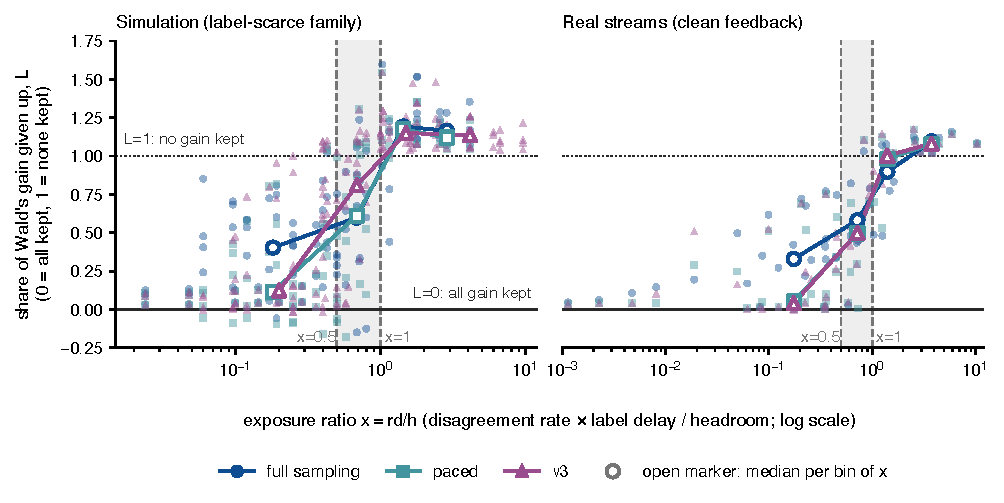
\includegraphics[width=\linewidth]{figures/fig_regime_map.pdf}
\caption{For the paced variants, median $L$, the share of the unconstrained rule's improvement given up, is small when $x=rd/h<0.5$ and close to 1 when $x\ge1$. Each point is one evaluated unit (regime or stream, shield arm, headroom $h$) where Wald with cutoff gains at least 10\% of the cost of never switching. Here $x$ is disagreement rate times label delay divided by headroom; $L=0$ means the whole gain is kept and $L=1$ that none is. Values $L<0$ mean the shield is cheaper than Wald, while $L>1$ means it costs more than never switching. Left: label-scarce simulation family; right: ten real streams with clean feedback. Open markers show bin medians for $[0,.5)$, $[.5,1)$, $[1,2)$ and $[2,\infty)$; lines join those medians and are not a fitted law. The shaded band marks $.5\le x<1$. Source: \texttt{exposure\_ratio\_test.json}.}
\label{fig:regime_map}
\end{figure}

A regression of $L$ on $\log x$ and the log labels per exposed round gives a positive coefficient on $\log x$ in all six fits (Appendix Table~\ref{tab:ols}), so the effect is not explained by label use. The test is correlational, and these units share tapes within a regime or stream.

In the registered simulation the default regimes have $r=\DefR$ and $d=\DefD$, so $x=\DefXTwelve$, \DefXTwenty{} and \DefXThirty{} at $R=12,20,30$, all in the retaining range. The pooled difference to Wald with cutoff at $R=20$ is \SimVsWaldDelta{} ([\SimVsWaldLo, \SimVsWaldHi], \SimVsWaldPct\% of its cost), and \OrigDelta{} on the 24 original regimes (\OrigPct\%). A label-scarce variant (v3) selected on simulation narrows the gap at large headroom and does not change the picture (Appendix~\ref{app:v3}).

\begin{table}[t]
\caption{Regime map: Spearman correlation of $x=rd/h$ with $L$, the share of the unconstrained rule's improvement given up, and median $L$ by bin of $x$. Source: \texttt{exposure\_ratio\_test.json}.}\label{tab:regime}
\centering\scriptsize
\resizebox{\linewidth}{!}{\begin{tabular}{@{}l r l r r r r@{}}
\toprule
 & clusters & Spearman$(x,L)$ [95\% CI] & \multicolumn{4}{c}{median $L$ by $x=rd/h$} \\
\cmidrule(lr){4-7}
Arm & & & $<.5$ & $.5$--$1$ & $1$--$2$ & $\ge 2$ \\
\midrule
simulation, full & 32 & 0.69 [0.55, 0.81] & 0.40 & 0.60 & 1.19 & 1.16 \\
simulation, paced & 32 & 0.73 [0.62, 0.82] & 0.11 & 0.61 & 1.17 & 1.12 \\
simulation, v3 & 32 & 0.78 [0.71, 0.83] & 0.12 & 0.81 & 1.15 & 1.14 \\
real, full & 8 & 0.80 [0.52, 0.97] & 0.32 & 0.46 & 0.87 & 1.11 \\
real, paced & 8 & 0.74 [0.50, 0.91] & 0.05 & 0.27 & 0.96 & 1.09 \\
real, v3 & 8 & 0.77 [0.55, 0.92] & 0.04 & 0.44 & 0.99 & 1.09 \\
\bottomrule
\end{tabular}
}
\end{table}

\section{Related work}
\paragraph{Conservative bandits and safe exploration.}
The closest line keeps performance above a baseline at all times. Conservative bandits require cumulative reward to stay above a fixed fraction of the baseline's, uniformly over time, in the stochastic and adversarial settings~\citep{wu2016conservative}; the idea extends to contextual linear bandits~\citep{kazerouni2017conservative}, reinforcement learning~\citep{garcelon2020conservative}, and combinatorial semi-bandits via interleaving~\citep{katariya2019conservative}. Our shield is in the same family: it deploys the risky action only if a worst-case check on the accumulated outcome passes.
The differences are the following. The constraint there is multiplicative in the baseline's reward and is checked on feedback observed immediately for the played arm; here the budget is an additive amount $R$ on realised harm that includes switching fees, and the challenger's loss is learned only through purchased labels that arrive after a delay or never, so the shield pays reserves for pending feedback and for the rollback. Sampling is design-based with a label budget, which is absent there. \citet{wu2016conservative} prove regret bounds and a lower bound on the regret cost of the constraint; we give a lower bound on the reserve itself (Proposition~\ref{prop:reserves}).

The most recent and closest work we found is Prudent-Banker~\citep{hu2026prudent}, which treats $K$-armed adversarial bandits with and without arbitrary, unknown delays. It attains worst-case pseudo-regret $\tilde O(\sqrt T+\sqrt D)$, with $D$ the total delay, together with $\tilde O(1)$ pseudo-regret against a designated safe baseline policy, using a restart threshold calibrated to the worst-case distortion caused by unobserved feedback. Its guarantees are on pseudo-regret, an expectation, rather than pathwise with high probability; it has no switching fee, no rollback and no label budget, since feedback arrives passively for every played round; and its lower bounds concern the regret guarantees rather than the reserve that a pathwise budget requires. We found no prior work that treats this combination in our search.

\paragraph{Bandits with knapsacks.}
Bandits with knapsacks maximise reward subject to global resource budgets, and the process stops when a resource is exhausted~\citep{badanidiyuru2013bandits,badanidiyuru2018bandits}. The label budget $B$ here is a resource of that kind. The difference is the constrained quantity: in bandits with knapsacks the resource consumption of a pulled arm is part of the feedback received when the arm is pulled, whereas our budget is on the harm of an action whose cost is revealed only through delayed, sampled or missing labels. The requirement is a pathwise guarantee on that harm at every round, with reserves for what is in transit, not a regret bound on reward.

\paragraph{Sequential testing in online experiments.}
Always-valid $p$-values and confidence intervals keep type I error under continuous monitoring of an A/B test, which removes the inflation from repeated peeking~\citep{johari2017peeking,johari2022always}. They are inference procedures for a treatment effect in a randomised experiment. Our budget is not a test of an effect: it bounds the realised harm of a sequence of interventions that a controller chooses and can reverse, under arbitrary drift and dependence, with delayed and sampled outcomes and switching fees. We use anytime-valid machinery for the same reason they do, to allow a decision at every round, but the target and the object bounded differ.

\paragraph{Safe policy improvement and confidence sequences.}
High-confidence off-policy evaluation and policy improvement give a lower confidence bound on a new policy's value before it is deployed~\citep{thomas2015hcope,thomas2015hcpi}. That is a one-shot certificate from logged data, with no sequential rollback and no pending feedback. Off-policy confidence sequences supply time-uniform bounds for contextual bandits and apply them to gated deployment~\citep{karampatziakis2021offpolicy}; they assess the new policy's value, whereas we bound the cumulative harm of the deployed sequence, fees included. Our width uses Bennett and exact-coin mixtures in the manner of time-uniform confidence sequences~\citep{howard2021time,waudbysmith2024betting}. Design-based confidence sequences for delayed outcomes monitor a counterfactual cumulative reward in randomised experiments~\citep{lindon2026design}; they show that inverse-propensity error is a martingale only in a suitable event-time filtration, which our settlement accounting avoids by booking unsettled rounds at worst case. They do not control an intervention.

\paragraph{Delayed feedback and switching costs.}
Online learning under delayed feedback shows that delay multiplies regret in adversarial problems and adds to it in stochastic ones~\citep{joulani2013delayed}. We do not target regret; delay enters as a reserve. Switching costs change the achievable regret rate under bandit feedback~\citep{cesabianchi2013switching}, and observation budgets interact with switching costs~\citep{cheng2023feedback}. These works compare to the best fixed action and impose no constraint on realised harm.

\paragraph{Label-efficient model selection and monitoring.}
Active model selection queries labels to identify a good model among pre-trained ones~\citep{karimi2021online,liu2024cams}. The objective is selection or regret, not a budget on harm, and there is no switching fee, rollback or delay. Tracking the risk of a deployed model with confidence sequences flags harmful shifts and tolerates delayed labels~\citep{podkopaev2022tracking}; it is an alarm, not a controller with a harm guarantee. A drift controller gates costly interventions on an online risk certificate and escalates to rollback~\citep{lamaakal2026drift2act}; its certificate is on the current window risk, not on cumulative intervention harm. A challenger-switching analysis studies when to train and evaluate a challenger on a growing dataset and whether to switch, with regret against a foresight oracle~\citep{digalakis2025challenger}. None gives a budget on the harm of a reversible promotion with fees under delayed, missing and sampled feedback, and none shows that the reserves are necessary.

\section{Limitations and conclusion}
The 14 real streams were used by earlier work, though no arm of this study was run or tuned on them before; each stream has few episodes, so per-stream intervals are wide or absent. The baselines are in-house heuristics or documented adapters rather than native-source reproductions, and the calibrated comparators of Section~\ref{sec:calib} are reported separately. Simulated and cached outcomes are exogenous (O1), so the study does not cover actions that change outcomes. The guarantee concerns harm against never switching with a quantity $R$ the user must choose, and it says nothing about whether the challenger is good. The label-scarce variant of the shield was designed after the real-stream run and evaluated there as a second look. The regime-map result is a correlational test of a prediction, not a theorem. The budget $R$ is a user input and the guarantee is only as meaningful as that choice; assumption (L) requires that both models' predictions are logged at serving time, which has a compute cost that we do not charge; and the real-stream delays and corruptions are simulated, so the real streams test the accounting on real losses, not on authentic label latency.

We bound the realised harm of reversible model promotion under delayed, missing and sampled feedback, with a shield that holds exactly the reserves that the matching lower bound shows are needed. The budget held in every registered and real run, the heuristics that approximate it did not, and the retention of the unconstrained rule's gain followed the exposure ratio the same bound predicts.

\section*{Broader impact statement}
The guarantee is relative to the status quo, never switching, and to the stated observation model. It does not say that the challenger is good, that the incumbent is safe or fair, or that the loss captures every harm of interest: a budget on average loss does not bound harm to a subgroup unless the loss is defined for it. It does not cover actions that change outcomes (O1), for example a promoted model that changes how users behave, nor labels that are themselves systematically biased. A budget set too high, or a violated assumption, would give false assurance. The method makes promotion more conservative and uses only losses that a team already logs, so we see a low risk of misuse.

\bibliography{refs}
\bibliographystyle{tmlr}

\appendix
\section{Remaining proofs}\label{app:proofs}
\subsection{Proposition~\ref{prop:nocert}}
Fix a certifier, which is a (possibly randomised) function $f$ of the observed history $\mathcal H_\tau$ through round $\tau$ and its private coins. We show that $\mathcal H_\tau$ has the same distribution under $\mathcal E^+$ and $\mathcal E^-$. Run the controller on both tapes with the same coins. A label requested at round $s$ is released at the start of round $s+d_s\ge s+d$, so a label visible at the start of round $\tau$ was requested at some $s\le\tau-d$, where the tapes agree in losses, flags and delays. The flags of every round up to $\tau$ coincide, and the controller's earlier actions and query decisions are functions of its past observations and coins. By induction over rounds, the actions, queries and released labels through $\tau$ coincide pathwise, hence $\mathcal H_\tau$ does. Therefore the probability of certifying is the same number $c$ under both tapes. The type I error on $\mathcal E^-$ is $c$ (since $P_{\tau,h}(\mathcal E^-)\le0$) and the type II error on $\mathcal E^+$ is $1-c$ (since $P_{\tau,h}(\mathcal E^+)>0$), so the sum is $1$. If the type I error is at most $\alpha$, then $c\le\alpha$, which is the probability of certifying on $\mathcal E^+$.

For existence, suppose the horizon $[\tau,\tau+h-1]$ contains $n>k$ disagreement rounds under a flag pattern fixed in advance. Let both tapes agree up to $\tau-d$ and give $Z=+1$ (respectively $-1$) on every disagreement round after $\tau-d$. Then $P_{\tau,h}(\mathcal E^+)=n-k>0$ and $P_{\tau,h}(\mathcal E^-)=-n-k<0$, and neither tape violates O1--O4. $\square$

\emph{Remark.} If the two histories had total variation distance $\varepsilon$ instead of zero, the same argument gives a sum of at least $1-\varepsilon$. The proposition is the standard indistinguishability argument; we include it so that the claim in the introduction is proved rather than asserted.

\subsection{Lemma~\ref{lem:bennett}}
Write $\xi_s=\chi_s(1-q_s/\pi_s)$ for monitored $s$. We work conditionally on the tape (losses, flags and delay mechanism, which may react to the past but not to the current coin), so the only randomness is the coins. Then $\chi_s$ and $\pi_s$ are predictable and $\E[q_s\mid\text{past}]=\pi_s$, so $\E[\xi_s\mid\text{past}]=0$ and $\mathrm{Var}(\xi_s\mid\text{past})=\chi_s^2(1/\pi_s-1)\le1/\pi_s-1$. Also $\xi_s\le b$: if $\chi_s\ge0$ then $\xi_s\le\chi_s\le1$; if $\chi_s<0$ then $\xi_s\le|\chi_s|(1/\pi_s-1)\le1/\pi_{\min}-1$. Bennett's inequality gives $\E[e^{\lambda\xi_s}\mid\text{past}]\le\exp(\phi(\lambda)(1/\pi_s-1))$, so $e^{\lambda M_t-\phi(\lambda)V_t}$ is a nonnegative supermartingale started at 1, and so is the $w$-mixture $\sum_\lambda w_\lambda e^{\lambda M_t-\phi(\lambda)V_t}$. By Ville's inequality the mixture stays below $1/\delta$ for all $t$ with probability at least $1-\delta$. On that event, for each $\lambda$, $\lambda M_t<\ln(1/(\delta w_\lambda))+\phi(\lambda)V_t$, so $M_t\le D_\delta(V_t)$. If $V_t=0$ every monitored round had $\pi=1$, hence $q=1$ and $M_t=0$. $\square$

\subsection{Attainment on the all-harm tape}
For the full-sampling shield with $\pi\equiv1$, all rounds disagreement rounds with $Z=-1$, and an inner rule that always proposes $a=1$, at the first promotion round $t=n$ (the $n$-th exposed round) $W_t=2k+n$ for every delay $d$, because each earlier exposed round contributes one unit whether pending ($P$) or resolved ($A$) and the current round contributes $g_t=1$. The shield therefore deploys for exactly the rounds $n\le R-2k$, that is $\lfloor R-2k\rfloor$ of them. Proposition~\ref{prop:reserves} limits a valid controller to $e\le R-2k$ disagreement rounds in a window of length $m\le d$, so the shield attains the bound whenever $d\ge\lfloor R-2k\rfloor$. For $d<\lfloor R-2k\rfloor$ the proposition says nothing about holds longer than $d$ (labels arrive during the hold). Appendix Table~\ref{tab:prop3} reports the simulated first-spell length in $12$ cells.

\subsection{Proposition~\ref{prop:price}}
During the first spell $N=1$, so $W_t=2k+\sum_{\text{released}}\chi_s+\#\text{pending}+g_t$. With fixed delay $d$ the pending rounds and the current round are among the last $d$ rounds, so their number is at most $d$, and the released rounds are a prefix of the exposed sequence. Hence $W_t\le2k+d-S_n$ for some $n$, with $S_n=y_1+\dots+y_n$. A forced rollback needs $W_t>R$, i.e.\ $S_n<-m$ for some $n$. If $m<0$ the bound $e^{-2\mu m}\ge1$ is trivial. For $m\ge0$ and $\theta=2\mu$, Hoeffding's lemma for $y_i\in[-1,1]$ gives $\E[e^{-\theta y_i}\mid\text{past}]\le e^{-\theta\mu+\theta^2/2}=1$, so $e^{-\theta S_n}$ is a nonnegative supermartingale, and Ville's inequality gives $\PP(\inf_nS_n\le-m)\le e^{-\theta m}=e^{-2\mu m}$. For $\pm1$ steps with $\PP(y_i=+1\mid\text{past})=p'\ge p>\frac12$, $\E[(q/p)^{y_i}]=p'q/p+(1-p')p/q$, with $q=1-p$, is decreasing in $p'$ and equals $1$ at $p'=p$, so $(q/p)^{S_n}$ is a supermartingale. Since $S_n$ is an integer, $S_n<-m$ means $S_n\le-(\lfloor m\rfloor+1)$, and Ville gives $((1-p)/p)^{\lfloor m\rfloor+1}$. $\square$

\subsection{Scope of the numerical checks}
The Proposition~\ref{prop:price} check uses 2000 runs per cell (per the design record), inner rule always-challenger, label budget not binding and no ride-out. In \PFourAbove{} of the \PFourCells{} cells the simulated frequency exceeds the bound at the point estimate; the largest excess is \PFourMaxZ{} binomial standard errors, so none is distinguishable from sampling noise. The forced rollbacks seen in beneficial regimes of the registered run are mostly outside the proposition, because there the label budget runs out and rounds are booked blind, and the inner rule starts further spells.

\section{Sharper bound with settlement}\label{app:v2}
\begin{lemma}[Exact coin mixture]\label{lem:coin}
For $x\in[-1,1]$ and rate $\pi$, $\E\exp(\lambda x(1-q/\pi))\le\exp(\psi(\lambda,\pi))$ with $\psi(\lambda,\pi)=\ln\max\{\pi e^{-\lambda(1/\pi-1)}+(1-\pi)e^{\lambda},\ \pi e^{\lambda(1/\pi-1)}+(1-\pi)e^{-\lambda}\}$. Moreover $\psi\ge0$ and $\psi(\lambda,1)=0$. With $\Psi_t(\lambda)=\sum_s\psi(\lambda,\pi_s)$ over the rounds included in $M$, and a finite grid with weights $w_\lambda$ (five values of $\lambda$ aimed at total variance $4,16,64,256,1024$, weights $1/5$), with probability at least $1-\delta$, for all $t$, $M_t\le D_t=\min_\lambda[\ln(1/(\delta w_\lambda))+\Psi_t(\lambda)]/\lambda$, and $D_t=0$ if no included round had $\pi<1$. Any per-round $\pi\in[\pi_{\min},1]$ is allowed.
\end{lemma}
\emph{Proof.} The function $x\mapsto\E\exp(\lambda x(1-q/\pi))$ is convex, hence maximal at $x=\pm1$, which gives the two terms. By Jensen the expectation is at least $\exp(\lambda\E[x(1-q/\pi)])=1$, so $\psi\ge0$; at $\pi=1$ the coin is deterministic, so $\psi=0$. Then $\exp(\lambda M_t-\Psi_t(\lambda))$ is a supermartingale, and the mixture and Ville's inequality finish as for Lemma~\ref{lem:bennett}. $\square$

\emph{Settlement.} Rounds with $\pi_s=1$ are accounted as before (worst case one while pending, then the exact $\chi_s$, no martingale term). For a round with $\pi_s<1$ fix a window $w\ge1$ (the declared delay if known, else a parameter). The round is \emph{unsettled} until $s+w$ and is booked at worst case $1$ regardless of its coin. At $s+w$ it settles: it enters $M$ (its $\psi$ is added to $\Psi$) and contributes $\chi_s/\pi_s$ if queried and released, $1/\pi_s$ if queried and unreleased, and $0$ if not queried. The settled set at time $t$ is the deterministic prefix $\{s\le t-w\}$ of the sampled rounds, so $M$ over settled rounds is the same martingale stopped at a deterministic time and Lemma~\ref{lem:coin} applies; unsettled rounds are bounded by $1$ pathwise. Validity does not depend on $w$. The check becomes
\begin{align*}
W_t=&\,k(N_{t-1}+\one\{a_{t-1}=0\})+k+[\text{blind}]+[\pi=1:\ \text{resolved}+\text{pending count}]\\
&+[\text{sampled, settled}:\ A_s+\text{unreleased }1/\pi]+[\text{sampled, unsettled count}]+g_t+D_t,
\end{align*}
and satisfies $H_t+k\le W_t$ on the event of Lemma~\ref{lem:coin}, so Theorem~\ref{thm:main} applies unchanged.

\emph{Label pacing.} On an exposed round the target rate is the labels remaining divided by $\max(\hat r(T-t+1),1)$, with $\hat r$ the running disagreement rate. If the target is at least $1$ the shield uses $\pi=1$; otherwise $\pi=\max(\pi_{\min},\text{target})$, or blind if no labels remain. If the paced choice fails $W_t\le R$ it escalates to $\pi=1$, and if that fails it rolls back. The blind-round variant additionally leaves a round blind when the headroom $R-W_t(\text{blind})$ is at least a margin.

\section{Protocols, seeds and tuning}\label{app:protocols}
\paragraph{Registered confirmation.}
Registered 2026-11-15 before any confirmation seed was opened; methods, arm specifications (18 frozen arms), metrics and decision rules are frozen at the registering commit, and the run was made once. Seeds 5303500000--5303500999 (1000 per regime, 30 regimes), disjoint from the earlier hypothesis blocks. Harm is $\sup_tH_t$ and a violation is $\sup_tH_t>R+10^{-9}$. Intervals are Wilson 95\% per regime ($n=1000$) and, for $\Delta J$, a seed-cluster bootstrap with 10{,}000 resamples of the equal-weight regime mean.
Hypotheses: C1 zero violations for the deterministic arms; C2 per-regime Wilson upper bound at most $.05$ for the paced arms; C3 for each of five comparators the worst-regime exceedance of $R=20$ has Wilson lower bound above $.05$; C4 pooled $\Delta J$ of the $R=20$ shield against Wald with cutoff has upper bound below 3\% and against never switching below $0$; C5 pooled $\Delta J$ against Wald with cutoff over the six stress regimes has upper bound below $0$; C6 each ablation at $R=12$ has a worst-regime violation Wilson lower bound above $.05$. All six were supported. The arms were chosen after looking at two exploratory development runs (seed offsets 30000--30999 and 40000--40999 within the development block 5301000000, pilot offsets 20000--20199, tuning offsets 0--5); the six stress regimes were specified before any F3 run.

\paragraph{Real-stream protocol.}
Pre-specified and run once on 2026-11-16 (EXPOSED\_STREAMS\_FROZEN\_CONFIG: every stream had been used by earlier work). Data: cached paired 0/1 losses with 2000 events per episode: airlines (50 episodes), bank (8), criteo (50), elec2 (4), openml\_ldpa (32), rialto (16), spam (1), uci\_occupancy (4), weather (3), appliances (6), beijing\_pm25 (14), bike\_hour (6), household\_power (20), metro (16). Delays: 24 (metro, beijing\_pm25, bike\_hour), 144 (appliances, household\_power), spam 50, weather 1, elec2 48, and 100 for the remaining streams. $T=2000$, $B=200$, $c_q=.05$, $k=5$, 20 policy seeds per episode (development block offsets 60000--60019). Budgets $R=2k+h$. Violation rates use Wilson intervals over runs, which are optimistic because runs in an episode share a tape; episode-cluster bootstrap intervals (10{,}000 resamples) are used for $\Delta J$, absent for streams with fewer than six episodes.

\paragraph{Baselines and tuning.}
Comparators and the inner rule are tuned by a 32-configuration random search on six tuning seeds over the 24 original regimes, with the same budget for every method. None is a native-source reproduction: Wald with cutoff is a documented adapter of an earlier Wald/lower-confidence-bound rule with discounting and a late-label cutoff; CUSUM, the e-process gate, the CUSUM rollback and the stop-loss are in-house heuristics.

\paragraph{Exposure-ratio test.}
The test script and its prediction were committed before its first run, using existing outputs only: the label-scarce family (fresh seeds 5301071000--5301071499) and the 14 real streams (clean). A unit is a regime or stream, an arm and a headroom, kept where Wald with cutoff gains at least 10\% of $J$(never). The regime or stream is the bootstrap cluster because units of one regime share tapes.

\paragraph{Label-scarce variant (v3).}\label{app:v3}
The v2 shield with a lower pacing floor and a wider mixture grid, selected among \VThreeNCand{} candidates on a 47-regime label-scarce simulation family ($T=2000$, $B=200$, $k=5$) at seed offsets 70000--70199, frozen, then evaluated on fresh seeds 5301071000--5301071499 (scarce), 5301072000--5301072299 (original regimes) and on the real streams as a second look (the streams had been seen once with the earlier arms). The best selection score was \VThreeBest, against a higher cost for the earlier paced arm on the same family. The pacing floor barely mattered. Tables~\ref{tab:v3s}--\ref{tab:v3r}.

\section{Simulator, regimes and real streams}\label{app:sim}
\subsection{How the simulator generates a tape}
A tape holds both potential losses of every round, drawn once per (regime, seed) and shared by every controller, so all arms are compared on identical tapes. A regime specifies a path $p_t$, the probability that the challenger is correct given a disagreement, the disagreement rate $r$, the dependence $\rho$, the shared-error rate $e_{\rm both}$, a delay mechanism and optional overrides of $k$ and $B$. Given these:
\begin{enumerate}
\item A latent stationary Gaussian process $u_t=\rho u_{t-1}+\sqrt{1-\rho^2}\,\varepsilon_t$ with $u_0\sim N(0,1)$ and $\varepsilon_t$ i.i.d.\ standard normal (an AR(1) Gaussian copula). The challenger is \emph{correct on disagreement} in round $t$ iff $\Phi(u_t)<p_t$, so its marginal probability of being correct is exactly $p_t$ while consecutive rounds are dependent with strength $\rho$.
\item The flag $g_t$ is Bernoulli$(r)$, independent over rounds.
\item On a disagreement round exactly one model errs: $\ell_t(0)=1$ iff the challenger is correct, and $\ell_t(1)=1-\ell_t(0)$, so $Z_t=\pm1$.
\item On an agreement round both models share one error draw, Bernoulli$(e_{\rm both})$, so $\ell_t(0)=\ell_t(1)$ and $Z_t=0$.
\end{enumerate}
Hence $Z_t\in\{-1,0,1\}$ and $\E Z_t=\mu_t=r(2p_t-1)$. The path $p$ is evaluated at $(t-\tfrac12)/T$. The delay applied to a label bought in round $t$ is drawn into the tape: a fixed $d$; a random draw from a list of values with given probabilities; \emph{informative}, $d$ plus an extra delay when the round is a disagreement on which the challenger is correct; \emph{informative adverse}, the same extra delay when the challenger is wrong; \emph{dropout}, with probability $p_{\rm drop}$ the label never arrives; \emph{adverse dropout}, the same only on disagreement rounds on which the challenger is wrong. The true path $p_t$ and $\mu_t$ are visible to the evaluator only and are never passed to a controller. The tape is seeded by (seed, a hash of the regime identifier) and the controllers' coins by (policy seed, a constant), so tape and coins are independent streams.

\subsection{The 30 regimes}
Table~\ref{tab:regimes_app} lists every regime with the path, disagreement rate, dependence, delay and overrides exactly as in the two configuration files (\texttt{regimes\_v1.json} and \texttt{regimes\_f3\_v1.json}). The 24 original regimes cover stationary null, benefit and harm, abrupt and gradual change, delayed or short-lived benefit, reversals and seasonality, dependence at four levels, informative and random delay, correlated errors and little disagreement, a high fee and scarce labels. The six stress regimes are described in Section~\ref{sec:exp}.

{\scriptsize
\begin{longtable}{@{}p{3.3cm}p{2.9cm}rr>{\raggedright\arraybackslash}p{2.4cm}>{\raggedright\arraybackslash}p{1.1cm}>{\raggedright\arraybackslash}p{2.7cm}@{}}
\caption{All 30 simulated regimes. $p(t)$ is the probability that the challenger is correct when the models disagree, given by knots $t/T$:$p$ (``steps'': constant from each knot; ``linear'': interpolated; evaluated at $(t-\tfrac12)/T$). $r$ is the disagreement rate, $\rho$ the lag-1 dependence of the latent Gaussian process, $d_t$ the label delay in rounds. Defaults: $r=.3$, $\rho=0$, $e_{\rm both}=.1$, delay fixed at 5, $k=3$, $B=60$, $c_q=.05$. Override lists departures from the defaults other than $r$, $\rho$ and the delay. Meaning is the description in the configuration file.}\label{tab:regimes_app}\\
\toprule id & $p(t)$ (knots $t/T$:$p$) & $r$ & $\rho$ & delay $d_t$ & override & meaning \\
\midrule
\endfirsthead
\multicolumn{7}{@{}l}{\emph{Table~\thetable{} (continued)}} \\[2pt]
\toprule id & $p(t)$ (knots $t/T$:$p$) & $r$ & $\rho$ & delay $d_t$ & override & meaning \\
\midrule
\endhead
\multicolumn{7}{@{}l}{\emph{24 original regimes} (\texttt{regimes\_v1.json})} \\
stationary\_null & steps 0:.5 & .3 & 0 & fixed 5 & none & no benefit anywhere (p=.5) \\
stationary\_better & steps 0:.7 & .3 & 0 & fixed 5 & none & challenger better throughout \\
stationary\_worse & steps 0:.3 & .3 & 0 & fixed 5 & none & challenger worse throughout \\
abrupt\_beneficial & steps 0:.5, .3:.75 & .3 & 0 & fixed 5 & none & challenger becomes better at .3T \\
abrupt\_harmful & steps 0:.7, .3:.3 & .3 & 0 & fixed 5 & none & challenger better, turns worse at .3T \\
gradual\_beneficial & linear 0:.5, .2:.5, .7:.75, 1:.75 & .3 & 0 & fixed 5 & none & ramp to challenger-better \\
gradual\_harmful & linear 0:.7, .2:.7, .7:.3, 1:.3 & .3 & 0 & fixed 5 & none & ramp to challenger-worse \\
delayed\_onset & steps 0:.5, .6:.8 & .3 & 0 & fixed 5 & none & benefit starts at .6T \\
short\_transient & steps 0:.5, .4:.85, .48:.5 & .3 & 0 & fixed 5 & none & benefit window of .08T \\
long\_persistent & steps 0:.5, .1:.8 & .3 & 0 & fixed 5 & none & benefit from .1T \\
multiple\_reversals & steps 0:.5, .15:.8, .35:.3, .55:.8, .75:.3 & .3 & 0 & fixed 5 & none & four reversals \\
seasonal\_recurrence & seasonal, $.8$ for the first .5 of each $.2T$ period, else $.4$ & .3 & 0 & fixed 5 & none & periodic benefit windows \\
dep\_rho\_0.0 & steps 0:.5, .3:.7 & .3 & 0 & fixed 5 & none & abrupt benefit, AR(1)-copula dependence rho=0.0 \\
dep\_rho\_0.5 & steps 0:.5, .3:.7 & .3 & .5 & fixed 5 & none & abrupt benefit, AR(1)-copula dependence rho=0.5 \\
dep\_rho\_0.8 & steps 0:.5, .3:.7 & .3 & .8 & fixed 5 & none & abrupt benefit, AR(1)-copula dependence rho=0.8 \\
dep\_rho\_0.95 & steps 0:.5, .3:.7 & .3 & .95 & fixed 5 & none & abrupt benefit, AR(1)-copula dependence rho=0.95 \\
informative\_delay & steps 0:.5, .3:.75 & .3 & 0 & 3, plus 12 if the label favours the challenger & none & labels favouring the challenger arrive later \\
correlated\_errors & steps 0:.5, .3:.75 & .12 & 0 & fixed 5 & $e_{\rm both}=.45$ & models err together; little disagreement \\
small\_disagreement & steps 0:.5, .3:.75 & .03 & 0 & fixed 5 & none & very small disagreement rate \\
late\_improvement & steps 0:.5, .85:.9 & .3 & 0 & fixed 5 & none & benefit starts at .85T \\
High switch fee & steps 0:.5, .3:.75 & .3 & 0 & fixed 5 & $k=30$ & switch fee 30 \\
label\_scarcity & steps 0:.5, .3:.75 & .3 & 0 & fixed 5 & $B=6$ & B=6 \\
random\_delay & steps 0:.5, .3:.75 & .3 & 0 & random on 1/3/8/20/40 with probabilities .3/.3/.2/.15/.05 & none & random heavy-tailed delays \\
dep\_null\_rho\_0.95 & steps 0:.5 & .3 & .95 & fixed 5 & none & global null with strong dependence \\
\midrule
\multicolumn{7}{@{}l}{\emph{6 stress regimes} (\texttt{regimes\_f3\_v1.json})} \\
adverse\_informative\_delay & steps 0:.7, .3:.3 & .3 & 0 & 3, plus 40 if the label is unfavourable to the challenger & none & labels unfavourable to the challenger arrive much later \\
label\_dropout & steps 0:.7, .3:.3 & .3 & 0 & 5; each label never arrives w.p. .3 & none & 30\% of requested labels never arrive \\
Adverse dropout & steps 0:.6, .3:.25 & .3 & 0 & 5; labels unfavourable to the challenger never arrive w.p. .6 & none & unfavourable labels dropped w.p. .6 \\
Bait reversal & steps 0:.85, .25:.15 & .3 & 0 & fixed 5 & none & challenger strongly better first quarter then strongly worse \\
dep\_harmful\_rho\_0.95 & steps 0:.35 & .3 & .95 & fixed 5 & none & worse challenger, strong dependence \\
dep\_bait\_rho\_0.95 & steps 0:.8, .3:.2 & .3 & .95 & fixed 5 & none & bait then harm, strong dependence \\
\bottomrule
\end{longtable}

}

\subsection{The 14 real streams}
Table~\ref{tab:streams} describes the cached streams. Each episode is a block of 2000 consecutive events, each with a 0/1 loss of the incumbent and of the challenger. All 14 streams were used by earlier work in the same programme, and no arm of this study was run or tuned on them before.

\emph{Five sprint streams} (metro, beijing\_pm25, bike\_hour, appliances, household\_power; UCI repository, licence CC BY 4.0). The documented construction is the same for all five: the table is cleaned and sorted chronologically with $n$ rows; the binary label is $y=\one[\text{target}>\text{median of the target over rows }[0,0.3n)]$; the scaler and the one-hot encoder are fitted on rows $[0,0.3n)$; the incumbent is a logistic regression (\texttt{max\_iter}$=300$, $C=1$) fitted on rows $[0,0.15n)$ and the challenger a histogram gradient boosting classifier (100 iterations, depth 4, learning rate $.1$) fitted on rows $[0,0.3n)$; episodes are $K=\min(20,\lfloor(n-0.3n)/2000\rfloor)$ consecutive non-overlapping blocks of 2000 rows starting at row $0.3n$; the loss is $\one[\hat y\ne y]$. The documented descriptive statistics show the challenger better in 56 of the 62 episodes of these five streams.

\emph{Nine atlas streams} (airlines, bank, criteo, elec2, openml\_ldpa, rialto, spam, uci\_occupancy, weather). The cache holds derived 0/1 loss vectors of an incumbent and a challenger. Seven are byte copies of loss files from an earlier registered real-data run, and openml\_ldpa and uci\_occupancy come from a later sensitivity study that built them with a chronological train-and-score pipeline. The cache documentation does not record the models, the training windows or, for three streams, the task, so we state none; ``not documented'' in the table means exactly that.

\emph{Delays.} The delay of each stream is a constant number of events taken from the earlier work (24 for metro, beijing\_pm25 and bike\_hour; 144 for appliances and household\_power; 50 for spam, 1 for weather, 48 for elec2; 100 for the rest). The label of event $t$ is released at event $t+d$ on the event clock. These are simulated constants: the streams carry no authentic label-release times, and no result here speaks to real label latency.

\begin{table}[t]
\caption{The 14 real streams. The task is binary. LR = logistic regression, HGB = histogram gradient boosting, with the training windows described above; ``not documented'' = not recorded in the cache documentation or the programme's dataset inventory. ``ep.'' = episodes of 2000 events (230 in all); delay in events, a simulated constant; ``inc. err.'' and ``chall. err.'' = mean 0/1 loss over all events of all episodes; ``disagr.'' = fraction of events on which the two losses differ (the exposure rate $r$); ``challenger'' = whether its mean loss is lower.}\label{tab:streams}
\centering\scriptsize
\resizebox{\linewidth}{!}{\begin{tabular}{@{}p{2.2cm}p{3.0cm}p{2.5cm}lrrrrrl@{}}
\toprule
stream & task (binary) & source & models (inc. / chall.) & ep. & delay & inc. err. & chall. err. & disagr. & challenger \\
\midrule
airlines & binary flight delay & OpenML 1169 & not documented & 50 & 100 & 0.388 & 0.427 & 0.172 & worse \\
bank & binary term-deposit subscription & UCI 222 & not documented & 8 & 100 & 0.210 & 0.599 & 0.782 & worse \\
criteo & not in the inventory & not in the inventory & not documented & 50 & 100 & 0.347 & 0.333 & 0.066 & better \\
elec2 & price direction & OpenML electricity-normalized & not documented & 4 & 48 & 0.195 & 0.191 & 0.060 & better \\
openml\_ldpa & not in the inventory & not in the inventory & not documented & 32 & 100 & 0.332 & 0.197 & 0.224 & better \\
rialto & 1-vs-9 image task & Losing mirror & not documented & 16 & 100 & 0.101 & 0.028 & 0.082 & better \\
spam & binary spam & Katakis spam stream & not documented & 1 & 50 & 0.424 & 0.095 & 0.351 & better \\
uci\_occupancy & not in the inventory & not in the inventory & not documented & 4 & 100 & 0.241 & 0.035 & 0.227 & better \\
weather & daily rain & Elwell-Polikar Offutt AFB & not documented & 3 & 1 & 0.252 & 0.213 & 0.114 & better \\
\midrule
metro & traffic volume above median & UCI 492 & LR / HGB & 16 & 24 & 0.360 & 0.047 & 0.360 & better \\
beijing\_pm25 & PM2.5 above median & UCI 381 & LR / HGB & 14 & 24 & 0.332 & 0.260 & 0.207 & better \\
bike\_hour & rental count above median & UCI 275 & LR / HGB & 6 & 24 & 0.276 & 0.115 & 0.258 & better \\
appliances & appliance energy use above median & UCI 374 & LR / HGB & 6 & 144 & 0.411 & 0.259 & 0.432 & better \\
household\_power & global active power above median & UCI 235 & LR / HGB & 20 & 144 & 0.316 & 0.250 & 0.246 & better \\
\bottomrule
\end{tabular}
}
\end{table}

\section{Comparators, inner rule and shield arms}\label{app:comp}
Every comparator and the inner rule is implemented in \texttt{baselines.py} and \texttt{comparators.py} of the supplement. Labels follow the programme's fidelity registry: a \emph{documented adapter} is an arithmetic port of a rule from an earlier study of the programme, re-expressed on the same interface and not the original code path; an \emph{in-house heuristic} is a textbook rule written for these experiments. None is a native-source reproduction, and none is called state of the art. All comparators see the same information as the shield: the released labels, the flag $g_t$ and their own coins.

\paragraph{Shared acquisition (paced).}
On a round with $g_t=1$, while labels remain and the late-label cutoff is open, the rule buys a label with probability $\min\{\max\{L/(\hat r\,(T-t)),\,.05\},\,1\}$, where $L$ is the number of labels left, $\hat r=(n_{\rm dis}+5)/(t+20)$ is the running disagreement rate with a prior of rate $.25$ and weight $20$, and $n_{\rm dis}$ the number of disagreement rounds so far. The \emph{late-label cutoff} with parameter $c$ stops buying once $t+d>T-\lfloor cT\rfloor$, so that labels that would arrive in the last $cT$ rounds are not purchased. Comparators buy labels whichever model is deployed.

\paragraph{Tuned Wald with cutoff (documented adapter; the inner rule of every shield arm).}
The rule keeps discounted counts $n\leftarrow\lambda n+1$ and $m\leftarrow\lambda m+\one\{Z>0\}$ over released labels with $Z\ne0$, processed in order of request. With $\hat p=(m+.5)/(n+1)$ and $\mathrm{se}=\sqrt{\hat p(1-\hat p)/(n+1)}$ it forms the quantile $q(\ell)=\mathrm{clip}(\hat p+z_\ell\,\mathrm{se})$, where $z_\ell$ is the standard normal quantile of level $\ell$. If the incumbent is deployed it uses level $\gamma$ (a lower bound on the probability that the challenger is right, since $\gamma<\tfrac12$), takes the advantage $2q-1$, and promotes when advantage times $\hat r\,(T-t)$ exceeds $k$, that is when the lower-bounded gain over the remaining horizon pays the fee. If the challenger is deployed it uses level $1-\gamma$ and the advantage $1-2q$ of the incumbent, and switches back under the same test. Parameters: discount $\lambda$, level $\gamma$, cutoff fraction.

\paragraph{CUSUM (in-house heuristic).}
A two-sided cumulative-sum detector on released $Z$, oriented so that positive values favour the model that is not deployed: $s\leftarrow\max\{0,s+y-\delta\}$ with $y=Z$ if the incumbent is deployed and $y=-Z$ otherwise; when $s>h$ it switches and resets $s$. Parameters: drift $\delta$, threshold $h$, cutoff fraction; paced acquisition.

\paragraph{E-process gate over Wald (in-house heuristic).}
The gate blocks every promotion until a betting e-process on released labels reaches $1/\alpha$: $W\leftarrow W(1+\lambda_gZ)$ over each released label, opening for good once $W\ge1/\alpha$. Under the global null of no benefit this has type I error at most $\alpha$ for the observed rounds. After opening, the inner Wald rule is unrestricted, so the gate carries a null-validity guarantee only and none about the cost of a switch.

\paragraph{CUSUM rollback (in-house heuristic).}
Wald with cutoff promotes. After each promotion the rule monitors the released labels of rounds requested since the promotion with a one-sided CUSUM on harm, $s\leftarrow\max\{0,s-Z-.1\}$, and forces a rollback when $s>h$ (we use $h=4$ and $h=8$); re-promotion is allowed. While deployed it buys a label on every disagreement round if labels remain.

\paragraph{Naive stop-loss (in-house heuristic).}
Wald with cutoff promotes. The rule sums the harm $A=\sum(-Z)$ of the released labels it bought while deployed, counts action changes $N$ (including the promotion being considered), and when $kN+A>R-k$ it rolls back and blocks the challenger for the rest of the run. It books no reserve for pending labels and no confidence width, which is why it is the obvious but invalid risk budget. It buys a label on every disagreement round while deployed.

\paragraph{Tuning.}
The inner rule, CUSUM and the gate are tuned by a 32-configuration random search on six tuning seeds over the 24 original regimes, with the same budget for every method and the objective of the mean over regimes of $J/J_{\rm never}$. The search spaces and the resulting frozen values are in Table~\ref{tab:comp}. The two rollback comparators and the stop-loss reuse the tuned Wald with cutoff and have no tuned parameters of their own. The frozen shield arms are in Table~\ref{tab:arms}. One arm, the blind-round variant, was frozen with a differently tuned inner rule; every other shield arm uses the inner rule of Table~\ref{tab:comp}.

\begin{table}[t]
\caption{Comparators: label, frozen parameters (from \texttt{f3\_confirmation\_arms\_v1.json}) and search space. Cutoff fractions are multiples of $T$. $\lambda$ is the Wald discount, $\gamma$ its level, $\delta,h$ the CUSUM drift and threshold, $\alpha,\lambda_g$ the gate level and bet size.}\label{tab:comp}
\centering\scriptsize
\begin{tabular}{@{}p{2.3cm}p{3.2cm}p{5.6cm}p{4.0cm}@{}}
\toprule
name & label & tuned or fixed parameters (frozen) & tuning space (32 random draws)\\
\midrule
never & in-house reference & none & none \\
wald\_cut & documented adapter & $\lambda=0.932$, $\gamma=0.219$, paced acquisition, cutoff 0.3$T$ & $\lambda\in[.9,.999]$, $\gamma\in[.05,.5]$, cutoff $\in\{.05,.1,.15,.2,.3\}T$ \\
cusum & in-house heuristic & $\delta=0.302$, $h=2.905$, paced acquisition, cutoff 0.15$T$ & $\delta\in[.02,.4]$, $h\in[1,12]$ (log-uniform), cutoff $\in\{\text{none},.05,\dots,.3\}T$ \\
gate\_wald & in-house heuristic & Wald part $\lambda=0.905$, $\gamma=0.414$, cutoff 0.1$T$; gate $\alpha=0.2$, $\lambda_g=0.5$ & Wald space, $\alpha\in\{.05,.1,.2\}$, $\lambda_g\in\{.1,.25,.5\}$ \\
cusum\_rb\_h4, \_h8 & in-house heuristic & inner: wald\_cut above; rollback threshold $h\in\{4,8\}$, drift $0.1$ & threshold fixed by arm, not tuned \\
stoploss\_R12, \_R20, \_R30 & in-house heuristic & inner: wald\_cut above; budget $R\in\{12,20,30\}$ & $R$ set by the user, not tuned \\
\bottomrule
\end{tabular}

\end{table}

\begin{table}[t]
\caption{Shield arms as frozen, with the inner rule each wraps. The label reserve is a fraction of $B$.}\label{tab:arms}
\centering\scriptsize
\begin{tabular}{@{}p{3.0cm}p{2.5cm}p{4.2cm}p{5.3cm}@{}}
\toprule
arm & variant & inner rule (tuned) & shield settings \\
\midrule
f3\_pi1\_R20 & full sampling & $\lambda=0.932$, $\gamma=0.219$, cutoff 0.3$T$ & $\pi=1$ on every exposed round, $\delta=0$, label reserve 0.25$B$; $R\in\{12,20,30\}$ \\
f3v2d\_R20 & paced, settlement & $\lambda=0.932$, $\gamma=0.219$, cutoff 0.3$T$ & $\pi_{\min}=0.5$, $\delta=0.05$, label reserve 0.25$B$, settlement window = declared delay (else 10); $R\in\{20,30\}$ \\
f3v2\_R20\_blind8 & blind-round & $\lambda=0.970$, $\gamma=0.283$, cutoff 0.05$T$ & $\pi_{\min}=1$ (so $\pi\in\{1,\text{blind}\}$), blind margin 8, label reserve 0.325$B$, window 5; $R=20$ \\
v3 (frozen in \texttt{f3\_v3\_frozen.json}) & label-scarce & wald\_cut as above & $\pi_{\min}=0.25$, label reserve 0.25$B$, no blind rounds, mixture grid up to total variance 4096, $\delta=0.05$ \\
\bottomrule
\end{tabular}

\end{table}

\section{Reproducibility and compute}\label{app:repro}
\paragraph{Reproducibility.}
The anonymised supplement contains the code (\texttt{src/shiftlab/paper3}), the configuration files named in this paper (the regime files, \texttt{f3\_confirmation\_arms\_v1.json}, \texttt{f3\_v3\_frozen.json}, the seed registry), the registration documents with the registering commit of the confirmation, the cached loss streams, the result files read by the table generator, and the run ledger. The registered confirmation is run with \texttt{run\_confirm.py --open-confirmation} and analysed with \texttt{analyze\_confirm.py}; the real-stream study with \texttt{run\_real.py} and \texttt{analyze\_real.py}; the checks of Propositions~\ref{prop:reserves} and~\ref{prop:price} with \texttt{check\_props.py}; the label-scarce variant with \texttt{select\_v3.py}, \texttt{run\_v3.py}, \texttt{run\_real\_v3.py} and their analysis scripts; the exposure-ratio test with \texttt{exposure\_ratio\_test.py}. Running \texttt{make\_tables.py} regenerates every table and every inline number of this paper from the result files, and \texttt{build.sh} rebuilds the PDF. Seeds are integers drawn from the blocks of the seed registry (smoke, development, model selection, confirmation), which are disjoint; the confirmation block is opened once, and the run refuses to start if its output directory already exists.

\paragraph{Compute.}
All experiments run on CPU only, with no GPU, in Python with multiple worker processes (up to $8$ for simulation and $6$ for the real-stream runs). Wall-clock times from the ledger are: registered confirmation (30 regimes, 18 arms, \NRunsPerArm{} runs per arm) \WallConfirm{} s; real-stream study (14 streams, 230 episodes, 20 policy seeds, three conditions, 22 arms) \WallReal{} s; label-scarce variant selection \WallVSel{} s, its fresh-seed evaluation on the scarce family \WallVScarce{} s and on the original regimes \WallVOrig{} s, and its second look at the real streams \WallVReal{} s. The \NLedgerStages{} stages in the ledger, including development and tuning, add up to about \WallTotalMin{} minutes. The ledger does not record the machine.

\section{Complete tables}
\begin{table}[t]\caption{All 18 frozen arms, pooled over 30 simulated regimes. $q_{95},q_{99}$, max are of $\sup_tH_t$.}\centering\small\begin{tabular}{@{}l r r r r r r@{}}
\toprule
Arm & $J$ & labels & $q_{95}$ & $q_{99}$ & max & deployed frac. \\
\midrule
Never switch & 71.53 & 0.0 & 0 & 0 & 0 & 0.000 \\
Wald with cutoff & 68.47 & 38.8 & 23 & 37 & 59 & 0.560 \\
CUSUM & 68.97 & 47.0 & 29 & 34 & 117 & 0.454 \\
E-process gate & 71.89 & 49.7 & 19 & 33 & 57 & 0.278 \\
CUSUM rollback ($h=4$) & 68.97 & 47.8 & 16 & 31 & 68 & 0.417 \\
CUSUM rollback ($h=8$) & 68.62 & 49.8 & 19 & 35 & 71 & 0.507 \\
Stop-loss ($R=12$) & 69.28 & 49.1 & 15 & 34 & 59 & 0.486 \\
Stop-loss ($R=20$) & 68.79 & 49.8 & 18 & 34 & 59 & 0.509 \\
Stop-loss ($R=30$) & 68.74 & 49.9 & 18 & 34 & 59 & 0.511 \\
Full shield ($R=12$) & 70.32 & 42.1 & 12 & 12 & 12 & 0.377 \\
Full shield ($R=20$) & 69.43 & 44.2 & 16 & 20 & 20 & 0.436 \\
Full shield ($R=30$) & 69.25 & 44.5 & 17 & 28 & 30 & 0.455 \\
Paced shield ($R=20$) & 69.80 & 37.8 & 13 & 16 & 22 & 0.366 \\
Paced shield ($R=30$) & 68.72 & 40.5 & 16 & 21 & 31 & 0.464 \\
Blind shield ($R=20$) & 69.18 & 40.0 & 14 & 17 & 20 & 0.418 \\
Ablation: no pending reserve & 70.29 & 44.1 & 14 & 29 & 46 & 0.422 \\
Ablation: no rollback reserve & 69.69 & 43.5 & 14 & 15 & 15 & 0.413 \\
Ablation: no width & 71.74 & 28.2 & 15 & 24 & 53 & 0.323 \\
\bottomrule
\end{tabular}
\end{table}
\begin{table}[t]\caption{Exceedance rate of $R=20$ by regime (1000 runs per cell).}\centering\scriptsize\resizebox{\linewidth}{!}{\begin{tabular}{@{}l r r r r r r r@{}}
\toprule
Regime & Wald & CUSUM & Gate & CUSUM-rb & Stop & Shield pi1 & Shield paced \\
\midrule
abrupt\_beneficial & 0.001 & 0.001 & 0.001 & 0.001 & 0.004 & 0.000 & 0.000 \\
abrupt\_harmful & 0.120 & 0.041 & 0.022 & 0.020 & 0.021 & 0.000 & 0.000 \\
adverse\_informative\_delay & 0.120 & 0.051 & 0.022 & 0.011 & 0.018 & 0.000 & 0.000 \\
Bait reversal & 0.034 & 0.003 & 0.001 & 0.000 & 0.000 & 0.000 & 0.001 \\
correlated\_errors & 0.000 & 0.000 & 0.000 & 0.000 & 0.000 & 0.000 & 0.000 \\
delayed\_onset & 0.000 & 0.003 & 0.010 & 0.003 & 0.002 & 0.000 & 0.000 \\
dep\_bait\_rho\_0.95 & 0.073 & 0.063 & 0.033 & 0.023 & 0.030 & 0.000 & 0.000 \\
dep\_harmful\_rho\_0.95 & 0.098 & 0.129 & 0.064 & 0.032 & 0.045 & 0.000 & 0.000 \\
dep\_null\_rho\_0.95 & 0.093 & 0.087 & 0.067 & 0.042 & 0.045 & 0.000 & 0.000 \\
dep\_rho\_0.0 & 0.000 & 0.001 & 0.001 & 0.000 & 0.001 & 0.000 & 0.000 \\
dep\_rho\_0.5 & 0.007 & 0.003 & 0.008 & 0.003 & 0.009 & 0.000 & 0.000 \\
dep\_rho\_0.8 & 0.031 & 0.027 & 0.023 & 0.014 & 0.024 & 0.000 & 0.000 \\
dep\_rho\_0.95 & 0.055 & 0.048 & 0.051 & 0.027 & 0.039 & 0.000 & 0.000 \\
Adverse dropout & 0.852 & 0.684 & 0.635 & 0.830 & 0.841 & 0.000 & 0.000 \\
High switch fee & 0.143 & 0.987 & 0.145 & 0.160 & 0.000 & 0.000 & 0.000 \\
gradual\_beneficial & 0.000 & 0.001 & 0.002 & 0.000 & 0.003 & 0.000 & 0.000 \\
gradual\_harmful & 0.075 & 0.018 & 0.022 & 0.031 & 0.032 & 0.000 & 0.000 \\
informative\_delay & 0.001 & 0.000 & 0.001 & 0.000 & 0.001 & 0.000 & 0.000 \\
label\_dropout & 0.207 & 0.075 & 0.036 & 0.064 & 0.073 & 0.000 & 0.000 \\
label\_scarcity & 0.000 & 0.000 & 0.000 & 0.000 & 0.000 & 0.000 & 0.000 \\
late\_improvement & 0.007 & 0.007 & 0.008 & 0.009 & 0.016 & 0.000 & 0.000 \\
long\_persistent & 0.000 & 0.000 & 0.000 & 0.000 & 0.000 & 0.000 & 0.000 \\
multiple\_reversals & 0.016 & 0.081 & 0.070 & 0.020 & 0.018 & 0.000 & 0.000 \\
random\_delay & 0.001 & 0.001 & 0.000 & 0.000 & 0.002 & 0.000 & 0.000 \\
seasonal\_recurrence & 0.009 & 0.017 & 0.036 & 0.006 & 0.012 & 0.000 & 0.000 \\
short\_transient & 0.018 & 0.012 & 0.009 & 0.016 & 0.020 & 0.000 & 0.000 \\
small\_disagreement & 0.000 & 0.000 & 0.000 & 0.000 & 0.000 & 0.000 & 0.000 \\
stationary\_better & 0.000 & 0.000 & 0.000 & 0.001 & 0.002 & 0.000 & 0.000 \\
stationary\_null & 0.006 & 0.013 & 0.011 & 0.007 & 0.010 & 0.000 & 0.000 \\
stationary\_worse & 0.011 & 0.005 & 0.000 & 0.000 & 0.000 & 0.000 & 0.000 \\
\bottomrule
\end{tabular}
}\end{table}
\begin{table}[t]\caption{Real streams, clean feedback, all 14 streams. ``viol./exceed'' lists runs above $R=24$ and $R=60$ for comparators and violations of the arm's own budget for budget arms.}\centering\scriptsize\resizebox{\linewidth}{!}{\begin{tabular}{@{}l r r r r r r r r@{}}
\toprule
Arm & $J$ & $\Delta J$ vs Wald & $\Delta J$ vs never & max harm & viol./exceed & labels & deployed & forced rb \\
\midrule
never & 602.19 & +179.6 & +0.0 & 0 & R24:0, R60:0 & 0.00 & 0.000 & n/a \\
wald\_cut & 422.60 & +0.0 & $-$179.6 & 175 & R24:456, R60:66 & 119.67 & 0.727 & n/a \\
cusum & 438.33 & +15.7 & $-$163.9 & 225 & R24:650, R60:131 & 147.11 & 0.677 & n/a \\
gate\_wald & 438.46 & +15.8 & $-$163.7 & 107 & R24:417, R60:114 & 156.06 & 0.605 & n/a \\
cusum\_rb\_h4 & 437.86 & +15.3 & $-$164.3 & 170 & R24:530, R60:112 & 165.56 & 0.666 & 0.90 \\
cusum\_rb\_h8 & 435.16 & +12.6 & $-$167.0 & 170 & R24:502, R60:109 & 168.00 & 0.693 & 0.27 \\
stoploss\_h14 & 439.33 & +16.7 & $-$162.9 & 65 & 298/3880 & 163.51 & 0.642 & 0.03 \\
stoploss\_h50 & 438.05 & +15.4 & $-$164.1 & 196 & 78/3880 & 167.85 & 0.688 & 0.01 \\
f3\_pi1\_h6 & 592.17 & +169.6 & $-$10.0 & 16 & 0/3880 & 108.25 & 0.182 & 1.22 \\
f3\_pi1\_h14 & 519.92 & +97.3 & $-$82.3 & 24 & 0/3880 & 140.02 & 0.448 & 1.13 \\
f3\_pi1\_h24 & 512.46 & +89.9 & $-$89.7 & 34 & 0/3880 & 147.89 & 0.503 & 1.04 \\
f3\_pi1\_h50 & 502.29 & +79.7 & $-$99.9 & 60 & 0/3880 & 155.32 & 0.553 & 0.67 \\
f3\_pi1\_h100 & 486.25 & +63.6 & $-$115.9 & 100 & 0/3880 & 158.17 & 0.587 & 0.43 \\
f3v2d\_h14 & 510.37 & +87.8 & $-$91.8 & 24 & 0/3880 & 125.84 & 0.430 & 0.93 \\
f3v2d\_h50 & 455.29 & +32.7 & $-$146.9 & 52 & 0/3880 & 145.43 & 0.622 & 0.59 \\
f3v2d\_h100 & 441.82 & +19.2 & $-$160.4 & 89 & 0/3880 & 150.44 & 0.666 & 0.28 \\
f3v2\_blind8\_h14 & 603.59 & +181.0 & +1.4 & 24 & 0/3880 & 118.99 & 0.178 & 1.66 \\
\bottomrule
\end{tabular}
}\end{table}
\begin{table}[t]\caption{Real streams, adverse dropout, all 14 streams.}\centering\scriptsize\resizebox{\linewidth}{!}{\begin{tabular}{@{}l r r r r r r r r@{}}
\toprule
Arm & $J$ & $\Delta J$ vs Wald & $\Delta J$ vs never & max harm & viol./exceed & labels & deployed & forced rb \\
\midrule
Never switch & 597.89 & +191.3 & +0.0 & 0 & R24:0, R60:0 & 0.00 & 0.000 & n/a \\
Wald with cutoff & 406.62 & +0.0 & $-$191.3 & 529 & R24:890, R60:447 & 121.43 & 0.831 & n/a \\
CUSUM & 414.03 & +7.4 & $-$183.9 & 363 & R24:889, R60:411 & 147.07 & 0.775 & n/a \\
E-process gate & 407.44 & +0.8 & $-$190.4 & 386 & R24:644, R60:304 & 155.05 & 0.767 & n/a \\
CUSUM rollback ($h=4$) & 416.46 & +9.8 & $-$181.4 & 529 & R24:921, R60:402 & 168.54 & 0.790 & 0.48 \\
CUSUM rollback ($h=8$) & 415.44 & +8.8 & $-$182.4 & 529 & R24:884, R60:429 & 170.55 & 0.813 & 0.08 \\
Stop-loss ($h=14$) & 414.87 & +8.2 & $-$183.0 & 529 & 886/4600 & 169.71 & 0.810 & 0.00 \\
Stop-loss ($h=50$) & 413.50 & +6.9 & $-$184.4 & 529 & 432/4600 & 170.54 & 0.818 & 0.00 \\
Full shield ($h=6$) & 590.98 & +184.4 & $-$6.9 & 16 & 0/4600 & 107.66 & 0.179 & 1.26 \\
Full shield ($h=14$) & 521.74 & +115.1 & $-$76.2 & 24 & 0/4600 & 138.75 & 0.460 & 1.46 \\
Full shield ($h=24$) & 508.98 & +102.4 & $-$88.9 & 34 & 0/4600 & 148.54 & 0.540 & 1.37 \\
Full shield ($h=50$) & 492.82 & +86.2 & $-$105.1 & 60 & 0/4600 & 159.88 & 0.616 & 0.93 \\
Full shield ($h=100$) & 476.27 & +69.7 & $-$121.6 & 110 & 0/4600 & 163.69 & 0.664 & 0.58 \\
Paced shield ($h=14$) & 518.95 & +112.3 & $-$79.0 & 24 & 0/4600 & 123.17 & 0.414 & 1.19 \\
Paced shield ($h=50$) & 447.24 & +40.6 & $-$150.7 & 58 & 0/4600 & 148.60 & 0.670 & 0.89 \\
Paced shield ($h=100$) & 431.58 & +25.0 & $-$166.3 & 101 & 0/4600 & 156.43 & 0.746 & 0.49 \\
Blind shield ($h=14$) & 601.12 & +194.5 & +3.2 & 24 & 0/4600 & 117.94 & 0.183 & 1.72 \\
\bottomrule
\end{tabular}
}\end{table}
\begin{table}[t]\caption{Real streams, adverse delay, all 14 streams.}\centering\scriptsize\resizebox{\linewidth}{!}{\begin{tabular}{@{}l r r r r r r r r@{}}
\toprule
Arm & $J$ & $\Delta J$ vs Wald & $\Delta J$ vs never & max harm & viol./exceed & labels & deployed & forced rb \\
\midrule
Never switch & 597.89 & +179.2 & +0.0 & 0 & R24:0, R60:0 & 0.00 & 0.000 & n/a \\
Wald with cutoff & 418.71 & +0.0 & $-$179.2 & 400 & R24:1017, R60:381 & 121.43 & 0.761 & n/a \\
CUSUM & 426.68 & +8.0 & $-$171.2 & 274 & R24:1050, R60:373 & 147.07 & 0.690 & n/a \\
E-process gate & 421.29 & +2.6 & $-$176.6 & 321 & R24:1142, R60:439 & 155.05 & 0.728 & n/a \\
CUSUM rollback ($h=4$) & 462.52 & +43.8 & $-$135.4 & 419 & R24:961, R60:317 & 167.56 & 0.620 & 0.65 \\
CUSUM rollback ($h=8$) & 460.46 & +41.8 & $-$137.4 & 419 & R24:980, R60:308 & 169.29 & 0.640 & 0.43 \\
Stop-loss ($h=14$) & 447.45 & +28.8 & $-$150.4 & 419 & 979/4600 & 169.23 & 0.672 & 0.01 \\
Stop-loss ($h=50$) & 446.77 & +28.1 & $-$151.1 & 419 & 305/4600 & 169.92 & 0.677 & 0.00 \\
Full shield ($h=6$) & 591.51 & +172.8 & $-$6.4 & 16 & 0/4600 & 107.93 & 0.179 & 1.25 \\
Full shield ($h=14$) & 524.20 & +105.5 & $-$73.7 & 24 & 0/4600 & 138.14 & 0.447 & 1.42 \\
Full shield ($h=24$) & 512.87 & +94.2 & $-$85.0 & 34 & 0/4600 & 148.10 & 0.529 & 1.28 \\
Full shield ($h=50$) & 498.64 & +79.9 & $-$99.2 & 60 & 0/4600 & 156.34 & 0.578 & 0.79 \\
Full shield ($h=100$) & 488.39 & +69.7 & $-$109.5 & 110 & 0/4600 & 160.42 & 0.603 & 0.51 \\
Paced shield ($h=14$) & 520.44 & +101.7 & $-$77.5 & 24 & 0/4600 & 122.92 & 0.412 & 1.22 \\
Paced shield ($h=50$) & 451.15 & +32.5 & $-$146.7 & 58 & 0/4600 & 146.51 & 0.653 & 0.80 \\
Paced shield ($h=100$) & 438.72 & +20.0 & $-$159.2 & 100 & 0/4600 & 151.33 & 0.699 & 0.40 \\
Blind shield ($h=14$) & 601.63 & +182.9 & +3.7 & 24 & 0/4600 & 117.94 & 0.187 & 1.75 \\
\bottomrule
\end{tabular}
}\end{table}
\begin{table}[t]\caption{Real streams, clean feedback, the two harmful streams.}\centering\scriptsize\resizebox{\linewidth}{!}{\begin{tabular}{@{}l r r r r r r r r@{}}
\toprule
Arm & $J$ & $\Delta J$ vs Wald & $\Delta J$ vs never & max harm & viol./exceed & labels & deployed & forced rb \\
\midrule
never & 598.09 & $-$8.8 & +0.0 & 0 & R24:0, R60:0 & 0.00 & 0.000 & n/a \\
wald\_cut & 606.84 & +0.0 & +8.8 & 120 & R24:167, R60:9 & 122.45 & 0.198 & n/a \\
cusum & 613.23 & +6.4 & +15.2 & 225 & R24:250, R60:24 & 149.22 & 0.196 & n/a \\
gate\_wald & 605.90 & $-$0.9 & +7.8 & 91 & R24:92, R60:11 & 157.06 & 0.090 & n/a \\
cusum\_rb\_h4 & 613.80 & +7.0 & +15.7 & 170 & R24:160, R60:21 & 136.09 & 0.159 & 0.44 \\
cusum\_rb\_h8 & 612.48 & +5.6 & +14.4 & 170 & R24:169, R60:21 & 139.44 & 0.189 & 0.02 \\
stoploss\_h14 & 608.62 & +1.8 & +10.5 & 55 & 76/1160 & 136.88 & 0.139 & 0.10 \\
stoploss\_h50 & 612.47 & +5.6 & +14.4 & 170 & 21/1160 & 139.48 & 0.189 & 0.00 \\
f3\_pi1\_h6 & 608.99 & +2.2 & +10.9 & 16 & 0/1160 & 92.84 & 0.010 & 0.54 \\
f3\_pi1\_h14 & 609.09 & +2.3 & +11.0 & 24 & 0/1160 & 97.98 & 0.064 & 0.62 \\
f3\_pi1\_h24 & 607.70 & +0.9 & +9.6 & 34 & 0/1160 & 105.27 & 0.118 & 0.44 \\
f3\_pi1\_h50 & 609.42 & +2.6 & +11.3 & 58 & 0/1160 & 111.76 & 0.135 & 0.39 \\
f3\_pi1\_h100 & 613.00 & +6.2 & +14.9 & 92 & 0/1160 & 117.35 & 0.142 & 0.22 \\
f3v2d\_h14 & 609.69 & +2.9 & +11.6 & 24 & 0/1160 & 94.86 & 0.041 & 0.59 \\
f3v2d\_h50 & 608.63 & +1.8 & +10.5 & 50 & 0/1160 & 106.47 & 0.137 & 0.34 \\
f3v2d\_h100 & 610.93 & +4.1 & +12.8 & 85 & 0/1160 & 110.45 & 0.148 & 0.36 \\
f3v2\_blind8\_h14 & 610.85 & +4.0 & +12.8 & 24 & 0/1160 & 112.51 & 0.021 & 0.55 \\
\bottomrule
\end{tabular}
}\end{table}
\begin{table}[t]\caption{Real streams, clean feedback, the twelve beneficial streams.}\centering\scriptsize\resizebox{\linewidth}{!}{\begin{tabular}{@{}l r r r r r r r r@{}}
\toprule
Arm & $J$ & $\Delta J$ vs Wald & $\Delta J$ vs never & max harm & viol./exceed & labels & deployed & forced rb \\
\midrule
never & 603.00 & +217.2 & +0.0 & 0 & R24:0, R60:0 & 0.00 & 0.000 & n/a \\
wald\_cut & 385.76 & +0.0 & $-$217.2 & 175 & R24:289, R60:57 & 119.12 & 0.832 & n/a \\
cusum & 403.35 & +17.6 & $-$199.7 & 118 & R24:400, R60:107 & 146.68 & 0.774 & n/a \\
gate\_wald & 404.97 & +19.2 & $-$198.0 & 107 & R24:325, R60:103 & 155.86 & 0.708 & n/a \\
cusum\_rb\_h4 & 402.67 & +16.9 & $-$200.3 & 108 & R24:370, R60:91 & 171.45 & 0.767 & 0.99 \\
cusum\_rb\_h8 & 399.70 & +13.9 & $-$203.3 & 96 & R24:333, R60:88 & 173.71 & 0.794 & 0.32 \\
stoploss\_h14 & 405.47 & +19.7 & $-$197.5 & 65 & 222/2720 & 168.84 & 0.743 & 0.02 \\
stoploss\_h50 & 403.17 & +17.4 & $-$199.8 & 196 & 57/2720 & 173.53 & 0.788 & 0.01 \\
f3\_pi1\_h6 & 588.81 & +203.1 & $-$14.2 & 16 & 0/2720 & 111.33 & 0.217 & 1.36 \\
f3\_pi1\_h14 & 502.08 & +116.3 & $-$100.9 & 24 & 0/2720 & 148.43 & 0.525 & 1.23 \\
f3\_pi1\_h24 & 493.41 & +107.7 & $-$109.6 & 34 & 0/2720 & 156.41 & 0.580 & 1.15 \\
f3\_pi1\_h50 & 480.86 & +95.1 & $-$122.1 & 60 & 0/2720 & 164.03 & 0.636 & 0.73 \\
f3\_pi1\_h100 & 460.90 & +75.1 & $-$142.1 & 100 & 0/2720 & 166.34 & 0.676 & 0.47 \\
f3v2d\_h14 & 490.51 & +104.8 & $-$112.5 & 24 & 0/2720 & 132.04 & 0.508 & 1.00 \\
f3v2d\_h50 & 424.62 & +38.9 & $-$178.4 & 52 & 0/2720 & 153.22 & 0.719 & 0.65 \\
f3v2d\_h100 & 408.00 & +22.2 & $-$195.0 & 89 & 0/2720 & 158.44 & 0.770 & 0.27 \\
f3v2\_blind8\_h14 & 602.13 & +216.4 & $-$0.9 & 24 & 0/2720 & 120.29 & 0.209 & 1.89 \\
\bottomrule
\end{tabular}
}\end{table}
\begin{table}[t]\caption{Mean cost $J$ per stream, clean feedback, $h=50$ ($R=60$).}\centering\scriptsize\begin{tabular}{@{}l r r r r r @{}}
\toprule
Stream & never & Wald+cutoff & stop-loss & shield full & shield paced \\
\midrule
airlines & 776.80 & 781.94 & 783.11 & 781.65 & 781.70 \\
bank & 419.38 & 431.73 & 441.84 & 437.19 & 435.56 \\
criteo & 693.92 & 681.04 & 683.29 & 683.25 & 683.28 \\
elec2 & 389.50 & 394.46 & 396.08 & 395.45 & 394.52 \\
rialto & 202.06 & 77.18 & 79.88 & 79.52 & 79.45 \\
spam & 849.00 & 212.55 & 213.85 & 472.40 & 213.30 \\
weather & 504.00 & 438.90 & 442.18 & 442.90 & 441.52 \\
appliances & 821.83 & 611.61 & 694.99 & 836.66 & 848.32 \\
beijing\_pm25 & 664.57 & 544.22 & 599.70 & 618.52 & 605.80 \\
bike\_hour & 552.83 & 254.37 & 252.68 & 335.70 & 259.68 \\
household\_power & 632.45 & 527.58 & 550.54 & 573.18 & 558.69 \\
metro & 719.88 & 115.64 & 118.50 & 371.02 & 161.61 \\
\bottomrule
\end{tabular}
\end{table}
\begin{table}[t]\caption{OLS of $L$ on $\log x$ and the log labels per exposed round.}\label{tab:ols}\centering\small\begin{tabular}{@{}l r r@{}}
\toprule
Arm & coef. of $\log x$ & coef. of $\log$(labels per exposed round) \\
\midrule
simulation, full & 0.23 & $-$0.06 \\
simulation, paced & 0.31 & +0.10 \\
simulation, v3 & 0.28 & +0.05 \\
real, full & 0.12 & $-$0.15 \\
real, paced & 0.15 & +0.02 \\
real, v3 & 0.16 & +0.01 \\
\bottomrule
\end{tabular}
\end{table}
\begin{table}[t]\caption{Proposition~\ref{prop:reserves}: simulated first-spell length of the full-sampling shield on an all-harm tape.}\label{tab:prop3}\centering\small\begin{tabular}{@{}r r r r r l l@{}}
\toprule
$d$ & $R$ & first spell & $\lfloor R-2k\rfloor$ & $\min(d,\lfloor R-2k\rfloor)$ & spell $=h$ & $d\ge h$ \\
\midrule
1 & 8 & 2 & 2 & 1 & yes & no \\
1 & 12 & 6 & 6 & 1 & yes & no \\
1 & 20 & 14 & 14 & 1 & yes & no \\
3 & 8 & 2 & 2 & 2 & yes & yes \\
3 & 12 & 6 & 6 & 3 & yes & no \\
3 & 20 & 14 & 14 & 3 & yes & no \\
5 & 8 & 2 & 2 & 2 & yes & yes \\
5 & 12 & 6 & 6 & 5 & yes & no \\
5 & 20 & 14 & 14 & 5 & yes & no \\
10 & 8 & 2 & 2 & 2 & yes & yes \\
10 & 12 & 6 & 6 & 6 & yes & yes \\
10 & 20 & 14 & 14 & 10 & yes & no \\
\bottomrule
\end{tabular}
\end{table}
\begin{table}[t]\caption{Proposition~\ref{prop:price}: simulated forced-rollback frequency against the ruin bound (2000 runs per cell); $z$ is the excess over the bound in binomial standard errors, zero when below.}\label{tab:prop4}\centering\small\begin{tabular}{@{}r r r r r r r@{}}
\toprule
$p$ & $d$ & $R$ & $m$ & forced rollbacks & bound & $z$ \\
\midrule
0.6 & 1 & 10 & +3 & 0.2035 & 0.1975 & 0.7 \\
0.6 & 1 & 12 & +5 & 0.0860 & 0.0878 & 0.0 \\
0.6 & 1 & 15 & +8 & 0.0220 & 0.0260 & 0.0 \\
0.6 & 1 & 20 & +13 & 0.0010 & 0.0034 & 0.0 \\
0.6 & 5 & 10 & $-$1 & 0.3970 & 1.0000 & 0.0 \\
0.6 & 5 & 12 & +1 & 0.1875 & 0.4444 & 0.0 \\
0.6 & 5 & 15 & +4 & 0.0530 & 0.1317 & 0.0 \\
0.6 & 5 & 20 & +9 & 0.0045 & 0.0173 & 0.0 \\
0.7 & 1 & 10 & +3 & 0.0345 & 0.0337 & 0.2 \\
0.7 & 1 & 12 & +5 & 0.0060 & 0.0062 & 0.0 \\
0.7 & 1 & 15 & +8 & 0.0005 & 0.0005 & 0.0 \\
0.7 & 1 & 20 & +13 & 0.0000 & 0.0000 & 0.0 \\
0.7 & 5 & 10 & $-$1 & 0.1670 & 1.0000 & 0.0 \\
0.7 & 5 & 12 & +1 & 0.0310 & 0.1837 & 0.0 \\
0.7 & 5 & 15 & +4 & 0.0025 & 0.0145 & 0.0 \\
0.7 & 5 & 20 & +9 & 0.0000 & 0.0002 & 0.0 \\
0.8 & 1 & 10 & +3 & 0.0045 & 0.0039 & 0.4 \\
0.8 & 1 & 12 & +5 & 0.0005 & 0.0002 & 0.7 \\
0.8 & 1 & 15 & +8 & 0.0000 & 0.0000 & 0.0 \\
0.8 & 1 & 20 & +13 & 0.0000 & 0.0000 & 0.0 \\
0.8 & 5 & 10 & $-$1 & 0.0685 & 1.0000 & 0.0 \\
0.8 & 5 & 12 & +1 & 0.0060 & 0.0625 & 0.0 \\
0.8 & 5 & 15 & +4 & 0.0005 & 0.0010 & 0.0 \\
0.8 & 5 & 20 & +9 & 0.0000 & 0.0000 & 0.0 \\
\bottomrule
\end{tabular}
\end{table}
\begin{table}[t]\caption{Label-scarce variant v3, scarce family (47 regimes), fresh seeds.}\label{tab:v3s}\centering\scriptsize\resizebox{\linewidth}{!}{\begin{tabular}{@{}l r l l l@{}}
\toprule
Arm & $J$ & $\Delta J$ vs Wald & $\Delta J$ vs never & violations \\
\midrule
Never switch & 433.81 & +92.98 [+92.64,+93.28] & +0.00 [+0.00,+0.00] & R24:0.000; R60:0.000; R110:0.000 \\
Wald with cutoff & 340.83 & +0.00 [+0.00,+0.00] & -92.98 [-93.30,-92.67] & R24:0.067; R60:0.004; R110:0.000 \\
Stop-loss ($h=50$) & 364.01 & +23.18 [+22.74,+23.63] & -69.79 [-70.29,-69.33] & 1374/23500 \\
Full shield ($h=50$) & 392.90 & +52.07 [+51.66,+52.49] & -40.90 [-41.27,-40.53] & 0/23500 \\
Paced shield ($h=50$) & 387.65 & +46.82 [+46.29,+47.34] & -46.15 [-46.66,-45.66] & 0/23500 \\
Full shield ($h=100$) & 382.59 & +41.76 [+41.37,+42.16] & -51.21 [-51.58,-50.84] & 0/23500 \\
Paced shield ($h=100$) & 357.55 & +16.72 [+16.33,+17.10] & -76.26 [-76.66,-75.85] & 0/23500 \\
Label-scarce shield ($h=50$) & 394.86 & +54.03 [+53.39,+54.67] & -38.95 [-39.59,-38.30] & 0/23500 \\
Label-scarce shield ($h=100$) & 355.31 & +14.48 [+13.99,+14.99] & -78.49 [-79.00,-77.98] & 0/23500 \\
\bottomrule
\end{tabular}
}\end{table}
\begin{table}[t]\caption{Label-scarce variant v3, original 30 regimes, fresh seeds.}\label{tab:v3o}\centering\scriptsize\resizebox{\linewidth}{!}{\begin{tabular}{@{}l r l l l@{}}
\toprule
Arm & $J$ & $\Delta J$ vs Wald & $\Delta J$ vs never & violations \\
\midrule
Wald with cutoff & 68.33 & +0.00 [+0.00,+0.00] & -3.25 [-3.46,-3.03] & R12:0.180; R20:0.065; R30:0.027 \\
Full shield ($R=12$) & 70.35 & +2.02 [+1.81,+2.24] & -1.22 [-1.44,-1.01] & 0/9000 \\
Full shield ($R=20$) & 69.50 & +1.16 [+0.97,+1.35] & -2.08 [-2.31,-1.86] & 0/9000 \\
Full shield ($R=30$) & 69.32 & +0.99 [+0.80,+1.17] & -2.26 [-2.49,-2.04] & 0/9000 \\
Paced shield ($R=20$) & 69.95 & +1.62 [+1.41,+1.83] & -1.63 [-1.85,-1.41] & 0/9000 \\
Paced shield ($R=30$) & 68.80 & +0.47 [+0.28,+0.67] & -2.77 [-3.00,-2.55] & 0/9000 \\
Label-scarce shield ($R=12$) & 73.07 & +4.74 [+4.49,+4.98] & +1.49 [+1.28,+1.70] & 0/9000 \\
Label-scarce shield ($R=20$) & 69.95 & +1.62 [+1.41,+1.83] & -1.63 [-1.84,-1.41] & 0/9000 \\
Label-scarce shield ($R=30$) & 68.82 & +0.49 [+0.30,+0.69] & -2.75 [-2.98,-2.53] & 0/9000 \\
\bottomrule
\end{tabular}
}\end{table}
\begin{table}[t]\caption{Label-scarce variant v3 on the real streams (second look), clean feedback, pooled.}\label{tab:v3r}\centering\scriptsize\begin{tabular}{@{}l r r r r@{}}
\toprule
Arm & $J$ & $\Delta J$ vs Wald & $\Delta J$ vs never & viol. \\
\midrule
f3\_pi1\_h50 & 502.29 & +79.7 & $-$99.9 & 0/3880 \\
f3v2d\_h50 & 455.29 & +32.7 & $-$146.9 & 0/3880 \\
v3\_h50 & 451.85 & +29.2 & $-$150.3 & 0/3880 \\
f3\_pi1\_h100 & 486.25 & +63.6 & $-$115.9 & 0/3880 \\
f3v2d\_h100 & 441.82 & +19.2 & $-$160.4 & 0/3880 \\
v3\_h100 & 435.38 & +12.8 & $-$166.8 & 0/3880 \\
\bottomrule
\end{tabular}
\end{table}

\end{document}
